\documentclass[11pt, a4paper]{memoir}
\usepackage[utf8]{inputenc}
\usepackage[english, science, dropcaps, hyperref, submissionstatement]{ku-frontpage}

% Redefining the abstract environment with a different text size
\let\oldabstract\abstract
\let\endoldabstract\endabstract


\renewenvironment{abstract}
  {\begin{oldabstract}\normalsize}  % Change the size here
  {\end{oldabstract}}
\renewcommand{\abstractnamefont}{\normalfont\Large\bfseries}


% Math-related packages
\usepackage{amsmath, amssymb, amsfonts, mathrsfs, latexsym, mathtools}
\usepackage{ntheorem}
\usepackage{tikz}
\usepackage[framemethod=TikZ]{mdframed}
\usepackage{centernot}
\usepackage{tikz-cd}
\usetikzlibrary{arrows.meta, decorations.pathreplacing, bending,patterns}

% Miscellaneous packages
\usepackage{csquotes}
\usepackage{enumitem}
\usepackage{lipsum}
\usepackage{float}
\usepackage{xcolor}
\usepackage{etoolbox}
\usepackage[most]{tcolorbox}
\tcbuselibrary{theorems, skins, breakable}
\usepackage{ulem}
\usepackage{microtype}
\usepackage{setspace}
\usepackage{graphicx, caption}
\usepackage{chngcntr}
\usepackage{cleveref}
\definecolor{emphcolor}{HTML}{901A1E} % Using kuRed

\newcommand{\coloremph}[1]{\textcolor{emphcolor}{\emph{#1}}}

\DeclareCaptionStyle{mystyle}{%
  font=it, % Italif font
  labelsep=space, % Use space instead of colon
  justification=RaggedRight % Left-align the caption
}
\captionsetup{style=mystyle}
\captionsetup{belowskip=-15pt}

\crefformat{footnote}{#2\footnotemark[#1]#3}
\counterwithout{figure}{chapter}

% Theorem-like environments with italicized text
\theoremstyle{break}
\theoremheaderfont{\normalfont\bfseries}
\theorembodyfont{\itshape} % Italicized text
\theoremseparator{.}

\newtheorem{thm}{Theorem}
\newtheorem{prop}{Proposition}
\newtheorem{cor}{Corollary}
\newtheorem{lem}{Lemma}

% Definition environment with non-italicized text
% Definition environment with non-italicized text
\theoremstyle{break}
\theoremheaderfont{\normalfont\bfseries\vspace{3pt}}
\theorembodyfont{\normalfont} % Non-italicized text
\theoremseparator{.}
\newtheorem{innerdefn}{Definition}

\newenvironment{defn}
  {\begin{innerdefn}}
  {\ensuremath{\circ}\end{innerdefn}}
  

\newtheorem{inneralg}{Algorithm}
\newenvironment{alg}{\begin{inneralg}}{\ensuremath{\circ}\end{inneralg}}  

% Alternative definition environment
\definecolor{kuRed}{HTML}{901A1E}
\definecolor{kuGray}{HTML}{666666}
\definecolor{lightKuGray}{HTML}{FFE8D1}

% Define the 'mydefinition' tcolorbox environment
\newtcolorbox[auto counter,number within=chapter]{mydefinition}[2][]{
  breakable, % Allows the box to break across pages
  colback=lightKuGray!80, % Background color for the entire box
  colframe=lightKuGray!80, % Frame color
  coltitle=black, % Text color for the title
  title={\textbf{Definition~\thetcbcounter\ (#2)\ #1}}, % Title with bold "Definition" and optional description
  fonttitle=\bfseries, % Make the title text bold
  enhanced,
  sharp corners,
  boxrule=1pt, % Width of the frame lines
  top=8pt, % Top space within the box (inside the frame)
  bottom=8pt, % Bottom space within the box (inside the frame)
  left=8pt, % Left space within the box (inside the frame)
  right=8pt, % Right space within the box (inside the frame)
  toprule=10pt,
  before=\vskip15pt,
  after=\vskip15pt,
  #1 % For specifying additional options
}

\theoremstyle{nonumberplain}
\theoremsymbol{\ensuremath{\square}} 
\newtheorem{proof}{Proof}

% Custom commands and math operators
\newcommand{\mN}{\mathbb{N}}
\newcommand{\mZ}{\mathbb{Z}}
\newcommand{\mQ}{\mathbb{Q}}
\newcommand{\mR}{\mathbb{R}}
\newcommand{\mD}{\mathbb{D}}
\newcommand{\mH}{\mathbb{H}}
\newcommand{\mC}{\mathbb{C}}
\newcommand{\mP}{\mathbb{P}}
\newcommand{\mF}{\mathbb{F}}
\newcommand{\abs}[1]{\left| #1\right|}
\newcommand{\norm}[1]{\left\lVert#1\right\rVert}
\newcommand{\indep}{\perp \!\!\! \perp}

\DeclareMathOperator{\pa}{pa}
\DeclareMathOperator{\de}{de}
\DeclareMathOperator{\nei}{ne}
\DeclareMathOperator{\bd}{bd}
\DeclareMathOperator{\nd}{nd}
\DeclareMathOperator{\an}{An}
\DeclareMathOperator{\supp}{supp}
\DeclareMathOperator{\rank}{rank}
\DeclareRobustCommand{\firstsecond}[2]{#2}

% Other settings
\setlength\arraycolsep{2 pt}
\setcounter{tocdepth}{2}
\setcounter{secnumdepth}{1}
\setlength{\jot}{8pt}

\assignment{Master's Thesis}

% The following are only needed if the \author, \title, \subtitle, and \date
% commands are not patchable. See the readme for more information.
% \frontpageauthor{Alex Author}
% \frontpagetitle{A concise but nevertheless\\precise and interesting title}
% \frontpagesubtitle{An intruiging subtitle}
% \frontpagedate{Submitted: \today}

\frontpagetitle{Causal Inference in Dynamical Systems}
\subtitle{Convergent Cross Mapping and Alternative Approaches}
\frontpageauthor{Rasmus Juhl Christensen}
\frontpagedate{Submitted: \today}
\advisor{Advisor: Niels Richard Hansen}
\frontpageimage{example.png}

\kupdfsetup{A concise but nevertheless precise and interesting title - An intruiging subtitle}{}{Alex Author}

\begin{document}
\begingroup
  \fontencoding{T1}\fontfamily{LinuxLibertineT-OsF}\selectfont
  \maketitle
\endgroup
\frontmatter

\begin{abstract}
This thesis investigates the identification of causal relationships in dynamical systems inspired by the Convergent Cross Mapping (CCM) method from the paper "Detecting Causality in Complex Ecosystems" by Sugihara et al., 2012. A key part of this work is establishing a framework for formulating causal models in dynamical systems and investigating how to analyze them via state space reconstruction methods. This thesis contains results in both a manifold and an attractor setting.\\
A significant portion of the thesis is dedicated to the theoretical derivations and details of results concerning causal identifiability. Central to this is the application of Takens' theorem for state space reconstruction, in that it gives conditions ensuring that the state space is encoded in observations of a single variable. This thesis investigates how this feature can be used for causal inference. The work compares and contrasts these findings with the established Granger causality framework, particularly looking at its limitations in deterministic systems and how state space reconstruction methods can remedy some of them.\\
In summary, the thesis aims to clarify how causality can be modeled and understood in dynamical systems. By applying and examining Convergent Cross Mapping and considering the interaction of deterministic and stochastic processes, this work aims to place CCM in a unified causal language, clarify assumptions and theoretical considerations, and thereby contribute with a refined description of what to look for when choosing state space reconstruction methods.
\end{abstract}

\vfill
\textit{Front page image generated by Chaoscope.}
\newpage

\addtocontents{toc}{\protect\setcounter{tocdepth}{-1}}

\tableofcontents

% Revert the change after the ToC
\addtocontents{toc}{\protect\setcounter{tocdepth}{3}}

\vfill
\noindent All code and data used in this project is available at \url{github.com/juhlc/speciale}.

\normalem

\newpage
\mainmatter

\chapter{Introduction}
Causality is a cornerstone of understanding the mechanics of systemic changes in various scientific domains, and at its core, causal inference addresses the intricate dance between correlation and causation. While correlation hints at a mutual relationship between two variables, causation pushes us into the territory of assertion — \textit{does one variable truly influence the other?} Traditional statistics employ randomization as a helpful tool. Imagine a medical scenario where a researcher can control who receives a treatment: If the researcher can ensure that it is perfectly random who receives the treatment and patients receiving the treatment consistently show improvement compared to those who do not, we can easily attribute that difference to the treatment. However, when variables are merely observed without that level of control, establishing causation becomes more complex. Causal statistics thus requires another level of statistical modeling because we want to reason about what happens when intervening in the process.\\\\
This thesis delves into the vibrant world of causal relationships in dynamical systems. Granger causality, a seminal and widely used concept in causal analysis of time series, yields one approach to causal inference in time-dependent data. It is based on the thoughts of \cite{Granger}, and it posits that if the past of a variable $C$ contains unique information about another variable $E$, the variable $C$ is said to \emph{Granger-cause} the variable $E$. This approach to causal inference is based on prediction, and at its core, it operates on the principle that cause precedes effect, which means that knowledge of the cause can enhance the predictability of the effect. However, while Granger causality offers a framework for assessing causality in probabilistic settings, it encounters challenges in deterministic systems. First, predictability no longer has the same meaning since it is not a signal clouded by noise but a feature of all variables. Dynamical systems, by nature, have variables that are interconnected and governed by underlying structures. This interconnectedness means that information about one variable can often be extracted from another due to the system's inherent dynamics rather than any direct causal link.\\\\
A case in point is the result from \cite{Takens}, which suggests that observing a single variable from a dynamical system might be sufficient to capture the entire system's dynamics. This interconnectedness can lead Granger causality to to identify causal links where none exist mistakenly. Enter now the deterministic systems' viewpoint: Instead of relying on simple prediction improvement as a marker of causality, we focus on the inherent information within variables. If variable 
$C$ causes variable $E$, then $E$ should encapsulate information about the dynamics of $C$. However, $C$ would not necessarily contain comprehensive information about $E$, as it would not include information about the dynamics of $E$ not imposed by $C$. This perspective flips Granger causality on its head: while Granger causality might predict the effect 
$C$ using the cause $E$, a deterministic viewpoint effectively suggests the opposite. \\\\
This subtle yet profound distinction reshapes our understanding of causality in dynamical systems. As we proceed, we will delve deeper into the theoretical underpinnings of this perspective, unpacking its implications and potential applications. In particular, this insight leads to the \emph{Convergent Cross Mapping} approach introduced by \cite{Sugihara}, which serves as both the motivational starting point and the culmination of the theoretical work based on Takens' theorem in this thesis. A detailed discussion of this approach is presented in Chapter \ref{chapTaken}.\\\\
However, while the deterministic paradigm offers a fascinating lens through which to understand causality, there is an inherent limitation. Real-world systems, especially in fields like economics, biology, and climate science, are rife with unpredictable fluctuations. These fluctuations cannot always be attributed solely to the endogenous dynamics of the system. No matter how meticulously one captures the deterministic dynamics, there will always be elements of seeming randomness and external influences that a purely deterministic model would struggle to account for. We return thus to stochastic processes. By reintroducing a stochastic element into our models, we can more faithfully represent the unpredictability and variability inherent in real-world systems. Stochasticity provides a framework to account for the  \enquote{noise} that is not explained by the deterministic components of a system. Moreover, it is a nod to the humility of our modeling efforts – recognizing that there are always aspects of complex systems that are beyond our current understanding or inherently random. 
In the subsequent chapters, we will delve deeper into the fusion of deterministic dynamics with stochastic processes using a mixture of simulation-based methods and theoretical considerations, seeking a harmonious balance that brings us closer to understanding the multifaceted nature of causality in dynamical systems.
\newpage
\section{An Example}
To illustrate the challenge of causal inference in complex dynamical systems, we will use a real-world example concerning interactions between anchovies, sardines, and sea surface temperature in the California Current ecosystem. This example serves as a backdrop for the more theoretical nature of the rest of this thesis. In keeping with the analysis of \cite{Sugihara}, we aim to use the same data for our analysis, but we do extend it by including data from the period 2012-2022 as well. The data consists of the following variables:
\begin{itemize}
\item Pacific sardine (\textit{Sardinops sagax}) California fish market catch landings recorded monthly in pounds from January 1928 up to and including December 2022. There are 12 months with redacted data.\footnote{\label{note1}Data from January 1928 up to and including December 2002 is obtained from \textit{ERDDAP} at \cite{oldData}, and data from January 2003 up to and including December 2022 is obtained directly from \cite{newData}.}
\item Northern anchovy (\textit{Engraulis mordax}) California fish market catch landings recorded monthly in pounds from January 1928 up to and including December 2022. There are 34 months with redacted data.\cref{note1} 
\item  Sea-surface temperature (SST) measured daily in $\text{C}^\circ$ as an average between temperatures measured at the two sites Scripps Pier Shore Station and Balboa Pier Shore Station from August 22, 1916, up to and including December 31, 2022. There are 458 days without any measurements at either site.\footnote{The data from Scripps Pier is maintained by \cite{Scripps} and covers the period from August 22, 1916, up to and including December 31, 2022. The data from Newport Pier is maintained by \cite{Newport} and covers the period from November 1, 1924, up to and including December 31, 2022.} 
\end{itemize}
Commercial landings data is considered confidential, and therefore, some landings recordings have been redacted due to insufficient data to summarize and maintain confidentiality.\footnote{This is a consequence of the California Fish and Game Code Section 8022. See: \url{https://wildlife.ca.gov/Conservation/Marine/Data-Management-Research/MFDE/User-Guide}} We will set landings in all months with redacted data to zero considering the reason for redaction. As for the temperature data, we impute missing data with surrounding data points on the reasoning that temperature probably does not vary significantly from day to day and that any specific day does not carry significant weight in yearly averages. Since the particular question is not of significant interest to the thesis itself and is only intended to illustrate the systems we intend to study, we shall not consider any implications of these choices in this thesis. For a comprehensive study of the inter dynamics of sardine and anchovy populations, we refer to \cite{Sardine}.\\\\
We will use the landings data as a proxy for the population size of sardines and anchovies. This, of course, does entail some problems since we have no measurements of the populations themselves, and will result in some uncertainty. However, we will disregard this discussion since it is not of inherent interest to the topic. To visualize the data, we plot the annual landings of sardine and anchovy alongside trend lines computed as the 3-year averages and the 3-year averages of the SST:
\begin{center}
	\begin{figure}[!ht]
		\includegraphics[width=\textwidth]{{"../r code/sardine"}.png}
		\caption{}
	\end{figure}
\end{center}
We observe a noticeable collapse in the sardine population in the 1960s, coinciding with a rapid growth of the anchovy population. There seems to be a significant negative correlation between sardine and anchovy landings in most of the 20th century. This phenomenon was not exclusive to the Califonia Current System, where the sardine ecosystem experienced an almost total ecological collapse as described in \cite{Sardine}. It was hypothesized in the 1970s that internal competition between the two species was a driving factor in the dynamics of the system; see, for instance, \cite{Compete}. In some places, the theory of interspecies competition led to suggested policies of subjecting the anchovy population to heavy fishing pressure in the hope that this would benefit the sardine ecosystem. Approaching the 21st century, the presumed negative correlation between sardine and anchovy populations seemed to disappear and even change sign, thus illustrating a feature of dynamical systems: variables can appear to be correlated, but over time, this correlation may vanish or change sign. This phenomenon is named \textit{mirage correlation} by \cite{Sugihara} and also serves as a reminder of the well-known fact that correlation does not imply causation. Moreover, we observe that the SST has risen sharply in recent years, consistent with global warming, which could impact findings based on this data.\\\\
To further illustrate the relationship between SST and the landings data, we transform the landings data to log-returns, i.e., the time series $(X_t)_{t\in T}\in \mR_+^T$ is transformed as follows
$$(X_t)_{t\in T} \mapsto \left(\log\left(1+\frac{X_t-X_{t-1}}{X_{t-1}}\right)\right)_{t\in T}\approx \left(\frac{X_t-X_{t-1}}{X_{t-1}}\right)_{t\in T}$$
The approximation on the right is valid when $(X_t-X_{t-1})X_{t-1}^{-1}$ is small. Thus, the log returns indicate the relative difference from year to year while shrinking very large positive values, which often appear in our data set. Below, we plot the log returns alongside 3-year averages and a scale of the 10-year average SST computed in each year as the average of the 10 previous years:
\begin{center}
	\begin{figure}[!ht]
		\includegraphics[width=\textwidth]{{"../r code/diff"}.png}
		\caption{}
	\end{figure}
\end{center}
The apparent patterns in the previous figure are significantly less noticeable now. A negative correlation between sardine and anchovy populations is less pronounced now, although we see some spikes in opposite directions around 1970 and 1980. More pronounced is the lower level of the averages of the SST in the 1960s and the return of the sardine population coinciding with the decline of the anchovy population and the return of higher average SSTs. The climate and ecological changes connected with the development in sea surface temperatures are also deemed to be driving the population changes in the analysis done by \cite{Sardine}. We observe that a potential causal relationship between temperature and sardine and anchovy landings is \textit{regime dependent} or \textit{state dependent}, thus revealing another feature of dynamical systems. The previous dynamic between temperature and population sizes seems to have disappeared in the recent warmer years, thus representing the phenomenon of mirage correlation. The State of California introduced legislation in the 1990s to protect the sardine population, which implemented restrictions based on temperature but later suspended in 2010 due to rising sea surface temperatures.\\\\
The log returns look fairly stationary over time, and one approach could be to analyze this data with standard techniques based on Granger causality in time series data. Let $X_t\in \mR^3$ denote the values of the log-return of sardine, the log-return of anchovy, and the average of sea surface temperature at time point $t$. We then introduce the VAR($p$)-model for this system:
$$X_t=A_1 X_{t-1}+A_2 X_{t-2}+\cdots + A_p X_{t-p}+u_t$$
where $A_1,\ldots, A_p\in \mR^{3\times 3}$ are coefficient matrices and $u_t$ is a noise term. The coefficient matrices can be estimated with OLS (the maximum likelihood estimator when assuming that $u_t$ is normally distributed and mean-zero), and we can get standard confidence intervals based on an assumption of asymptotic normality. We see that the matrices model the influence of past values of all variables on the present values of the variable in question. For now, we will cautiously endow this influence with a causal interpretation, although the nuances of this interpretation are yet to be made explicit. At the very least, we will take it as an indication of a possible causal link.\\\\ 
We have to choose the parameter $p$, specifying the number of lags in the model. This choice can be made by choosing the model according to a minimal information criterion like AIC. Fitting a VAR(1) model with first-differenced temperature data to the data yields an estimate of $-2.6$ of the coefficient from temperature to anchovies and an estimate of $17.9$ of the coefficient from temperature to sardines. The remaining coefficients for sardine and anchovy are all estimated to be $0.0$. No coefficient is significant at a 95\% level, but this is expected due to the small sample size. However, this does indicate that temperature might positively influence the sardine population and negatively influence the anchovy population. We are looking at averages of temperature over a 10-year period; any window of averaging in the range from 5 to 10 years does not change the sign and size of the estimates significantly, but when looking at the yearly averages of temperature alone, we no longer get estimates that do not round to 0. This shows that the indication is not just a happy accident, although we lack the power to say anything definitively.\\\\ 
However, these results do not exploit some of the properties of the dynamical systems we observed and discussed above, and the present approach requires some data manipulation to use the standard econometric methods. Notice, for instance, that a VAR($p$)-model under standard assumptions entails a stationary time series. Therefore, we must look for transformations of our time series yielding stationarity or at least something reasonably modeled with a stationary time series. In this example, we solve this by a standard transformation, but it is a model assumption that needs addressing. We will use these assumptions as an inspiration for the work that we will now undertake.


\chapter{Stochastic Causal Models}
We start by setting up the basic scenario that we wish to explore. In general, we will, in this thesis, imagine that we have to deal with a set of real variables
$$X=(X^1,\ldots, X^d)$$
and we imagine that we collect data points for each variable in some fixed time window 
$$X_1,\ldots, X_T$$
We now wish to use this data to model what happens with our variables in the future if some variables were subjugated to some \emph{exogenous} forcing, meaning that we want a model to directly allow for interventions on some variables not arising from the model itself and describe the down-stream consequences for the remaining variables in the system.\\[5pt]
In this chapter, we will examine a probabilistic approach to this problem, and therefore, we invoke the framework of random variables:
\begin{mydefinition}{Time Series}
Let $(\Omega,\mathcal{E},\mP)$ be a probability space. We shall call $(X_t)_{t\in \mZ}=(X_t^{1},\ldots,X_{t}^d)_{t\in \mZ}$ a \emph{$d$-dimensional discrete time series}, where $X_t^j:\Omega\to \mR$ is a random variable and the observation of the $j$th variable of $X$ at time $t$.\\[5pt]
We shall call $(X_t)_{t\in \mR}=(X_t^{1},\ldots,X_{t}^d)_{t\in \mR}$ a \emph{$d$-dimensional continuous time series}, where $X_t^j:\Omega\to \mR$ is a random variable and the observation of the $j$th variable of $X$ at time $t$.\\[5pt]
We will call $t\mapsto X_t$ the \emph{sample path of $X$}.
\end{mydefinition}
When we move to the dynamical systems approach in the next chapter, it is standard to use the terminology \enquote{trajectory} in place of \enquote{sample path}. We will imagine our data set as being realizations of our set of random variables at a finite set of time stamps, that is
$$X_{t_1}(\omega),\ldots,X_{t_n}(\omega),\quad n\in \mN$$
In this chapter, we will follow three main lines of thought. The first is to introduce functional assignments as a way of modeling the interaction structure between variables and, in particular, of modeling causality; the second is to introduce a graphical framework as a way of keeping track of the dependencies between variables; and the final is to exploit time-homogeneity of the data to allow for inference of the graph structure in the model. We will follow a similar recipe in the next chapter, moving to a dynamical systems approach. This chapter takes most of its inspiration from the theory of causal graphical models as pioneered by \cite{Spirtes} and \cite{Pearl}, and, of course, inspired by the work of \cite{Steffen}. We start by moving from our soft notion of cause and effect to a precise mathematical concept.
\section{A Simple Causal Model}
In this thesis, our main approach to causality is to model causal links via functional assignments. To illustrate, we introduce the \textit{Structural Causal Model (SCM)} in the terminology of \cite{Peters}, which in its most simple form can be formulated for two variables as
\begin{align*}
C&\coloneqq N_C\\
E&\coloneqq f(C,N_E)
\end{align*}
where $N_C,N_E$ are independent random variables and $f$ a deterministic function. In this case, we denote $C$ the cause and $E$ the effect. We notice that an SCM entails a unique joint distribution of $C$ and $E$. An obvious deficiency is that the representation above is not unique in the sense that varying the function and noise terms can generate models that entail the same distributions and imply the same effects of an intervention. However, this can be somewhat resolved by imposing distributional constraints on the noise terms and how $f$ depends on the variables.\\[5pt]
We shall think of these expressions as assignments and not merely equations fulfilled by the variables of the system. By this, we mean that we think of $E$ being \textit{generated} as the functional expression of $C$ and a noise term and not as fulfilling this property by accident, from an equilibrium condition, or something else along those lines. In principle, this is not mathematically relevant, but it guides how we think of interventions in the model. We will think of an intervention on a variable as overwriting its assignment: introducing a new distribution of $C$, say $N_C'$ independent from $N_E$, then induces the \emph{postintervention SCM}
\begin{align*}
C&\coloneqq N_C'\\
E&\coloneqq f(C,N_E)
\end{align*}
with the idea being that the effect depends on the cause via the same functional expression, unchanged by the intervention. If we were to intervene on the effect, we would overwrite the assignment of $E$, and the postintervention SCM would, in this case, take the form:
\begin{align*}
C&\coloneqq N_C\\
E&\coloneqq g(C,N_E')
\end{align*} 
with $g$ a new assignment function. In this model, one feature of causality is that intervening on effects is without consequence for the corresponding causes, while intervening on causes can produce changes in the effects but not in the functional relationship. The insistence on the assignment interpretation has the following reasoning:
If we believe these equations to be the result of an equilibrium, then we would not expect an intervention on $C$, such as fixing its value to $C\coloneqq c$, to necessarily produce the effect that $E$ is now given by $E\coloneqq f(c,N_E)$ - a reasonable assumption of an equilibrium model would be that it describes the mechanics that determines a new equilibrium. On the other hand, if we interpret these expressions as assignments, this should be the expectation under the model.\\[5pt]
Our fundamental approach to modeling time series will be the same. Nothing precludes us from letting $C,E$ be time-series and using this basic model. One drawback is that we might be interested in modeling what happens between multiple variables, thus motivating an extension to multiple variables. A more serious drawback is that we want to be more explicit in modeling the time-dependence structure of the data. Before moving to these two extensions, we will use this toy example to highlight the problem of \emph{identifiability} in causal models. This thesis will tackle the problem of trying to infer if a given variable is the cause of another. Therefore, we consider the \emph{causal direction} of the SCM as unknown: we might as well have $X$ and $Y$ flipped in our SCM \emph{a priori}. Therefore, we will focus in this thesis on giving conditions ensuring the identifiability of causal directions in a set of variables. We will mainly consider this from a theoretical angle, in the sense that we will consider a structure identifiable if we can derive it from constraints satisfied by the variables in the model. The practical side of checking whether these constraints are satisfied will be given less importance.\\[5pt]
To illustrate the necessity of more structure in our model, we illustrate the problem of identifiability in this simple SCM: If we assume $N_E$ is degenerate, i.e., $N_E\coloneqq e$ (a.s.), and $f$ is invertible in its first argument, i.e., $x\mapsto f(x,e)$ is invertible, then $E$ is the cause in the SCM
\begin{align*}
E&\coloneqq N_E'\\
C&\coloneqq f_x^{-1}(E,N_C')
\end{align*}
when $N_E'$ shares distribution with $E$ in the previous SCM and $N_C'$ is degenerate.  We can let $f_x^{-1}$ be defined on two arguments such that for the value of $N'_C$ in the second coordinate, it yields the inverse of $x\mapsto f(x,e)$. In this case, we cannot identify the direction of a causal link. Of course, one could object that this model encodes a deterministic relationship between our variables and that this counterexample is too simple to be interesting. We will return to the problem of deterministic relationships, but we note that this is not the issue here. This argument generalizes: If we consider the conditional cumulative distribution function $F_{Y|x}(y)\coloneqq \mP(Y\leqslant y\mid X=x)$ and define
$$f_Y(x,n_Y)\coloneqq F^{-1}_{Y|x}(n_Y)=\inf\{y\in \mR: F_{Y|x}(y)\geqslant n_Y\}$$
then we need only let $N_Y$ be uniformly distributed on $[0,1]$ and independent of $X$ for the above SCM to entail the distribution $\mP_{(X,Y)}$. We record this result as follows:
\begin{thm}[Non-Uniqueness of Causal Directness]
For every joint distribution\footnote{The simple proof requires the existence of conditional distributions, so we will assume this here. In fact, the theory is usually built while implicitly assuming that the distribution has a joint density.} of random variables $\mP_{(X,Y)}$, there is an SCM
$$Y=f_Y(X,N_Y),\quad X\indep N_Y$$
where $f_Y$ is a measurable function and $N_Y$ a real-valued noise variable.\\ \cite{Peters}
\end{thm}
We discuss this result not for its immediate relevance to the main topic of the thesis but to highlight the trickery of causal concepts and the weight our model assumptions will have to carry. A typical solution is to assume additive noise, which does yield identifiability under some regularity conditions; see \cite{ANM1} or \cite{ANM2}. Such results illustrate that with the right amount of structure and assumptions, we can render the causal direction perfectly identifiable and thus move the problem of causal discovery into the realm of practical considerations. There exists a plethora of machine learning methods capable of reliably estimating even very complex functions; thus, the question becomes one of checking an additive noise assumption, making sure that the random variables are not governed by a law exceptional to the result above, and dealing with the uncertainty inherited from finite sample sizes. In this section, we have provided a sketch for an approach to causality that we will repeat in this chapter and the entire thesis: introduce a causal model via functional assignments, introduce assumptions on the model, and derive an identifiability result.
\section{Graphical Models}\label{graphmod}
We will now introduce graphs to keep track of the causal structure in a network of variables. This will serve us both in discussing multivariate SCMs and also when introducing and discussing causal models of dynamical systems. We introduce more general graph concepts here than we will need in the SCM approach. This serves a dual purpose: 1) the generalization allows us to capture feedback between variables in graphical models, and 2) we have enough terminology to formulate the models in subsequent chapters. We introduce the following graph terminology:
\begin{mydefinition}{Graph Terminology}
Consider a \emph{graph} $\mathcal{G}=(\mathcal{V},\mathcal{E})$ with $\mathcal{V}$ the set of \emph{vertices} and $\mathcal{E}\subset \mathcal{V}\times \mathcal{V}$ the set of \emph{edges}.\\[5pt]
We distinguish \textit{directed} ($-$) and \textit{undirected} edges ($\to$): For $u,v\in \mathcal{V}$, we write $u-v$ if $(u,v),(v,u)\in \mathcal{E}$, and $u\to v$ if only $(u,v)\in \mathcal{E}$. \\[5pt]
If $u\to v$, we call $u$ a \emph{parent} of $v$, and we denote by $\pa(v)$ the set of parents of $v$. If $u-v$, we call $u$ a \emph{neighbor} of $v$, and we denote by $\nei(v)$ the set of neighbors of $v$. We define the \emph{boundary} of $v$ as $\bd(v)=\pa(v)\cup \nei(v)$, and for a subset $A\subset \mathcal{V}$, we define the parents, neighbours and boundary of $A$ as
\begin{align*}
\pa(A)&=\bigcup_{v\in A}\pa(v)\setminus A\\
 \nei(A)&=\bigcup_{v\in A}\nei(v)\setminus A\\
 \bd(A)&=\bigcup_{v\in A}\bd(v)\setminus A
\end{align*}
A \emph{chain} in $\mathcal{G}$ is a sequence of vertices $v_1,\ldots, v_n$ ($n \geqslant 2$) satisfying that for all $j=1,\ldots,n-1$, we have $v_{j+1}\in \bd(v_j)$ or $v_{j}\in \bd(v_{j+1})$, and a \emph{path} is a chain  where only $v_{j+1}\in \bd(v_j)$ is allowed. A graph is \emph{connected} if any two vertices are contained in a path. A \emph{directed path} is a path for which all edges between the vertices are directed. A \textit{partially directed cycle} in $\mathcal{G}$ is a cycle with at least one directed edge, that is a path $v_1,\ldots, v_n$ ($n \geqslant 3$) with $v_1\in \bd(v_n)$ and $v_{j+1}\to v_j$ for some $j$.\\[5pt]
For $A\subset V$, we call $A$ an \emph{ancestral set} if for all $\alpha\in A$ and  $\beta \in \mathcal{V}$ for which there exists a partially directed path from $\beta$ to $\alpha$ in $\mathcal{G}$, we have $\beta \in A$. We let $\an(A)$ denote the smallest ancestral set containing $A$, and $\an(\mathcal{G})$ the set of ancestral sets in $\mathcal{G}$.\\[5pt]
For $A\subset V$, $\mathcal{G}_A$ denotes the subgraph of $\mathcal{G}$ with $A$ as vertex set and all edges inherited from $\mathcal{G}$, and we say it is the subgraph \emph{induced} by $A$. We call a graph \emph{complete} if there is an edge (directed or undirected) between every pair of vertices, and we call a maximal complete subgraph $\mathcal{G}_A$for a \emph{clique}.\\[5pt]
A \emph{chain component} is a connected subgraph of $\mathcal{G}$ containing only undirected edges, and a \emph{minimal complex}  is an induced subgraph $\mathcal{G}_A$ with two distinguished nodes $a,b$ for which $\mathcal{G}_{A\setminus \{a,b\}}$ is a chain component and no path in $\mathcal{G}_A$ contains both $a$ and $b$. A minimal complex can be drawn as
$$a\to v_1-\cdots-v_n\gets b$$
The graph obtained from $\mathcal{G}$ by removing the direction on all edges and adding edges between the distinguished nodes for all minimal complexes in $\mathcal{G}$ is called the \emph{mutualized graph of $\mathcal{G}$},\footnotemark\ and we denote it $\mathcal{G}^m$.\\[5pt]
We say that $\mathcal{G}$ is a \emph{chain graph} if it contains no partially directed cycles, and if further, it contains no directed edges, we say $\mathcal{G}$ is a \emph{directed acyclic graph (DAG)}.
\end{mydefinition}
\footnotetext{This terminology is an invention of me, the author, to avoid the term \enquote{moralized graph}, which is standard terminology but personally considered outdated.}
We will implicitly assume our graphs to be finite, meaning that there are only finitely many vertices. However, this is not a necessary condition, and sometimes, it can be illuminating to think in infinite graph structures. However, all results in this chapter are to be interpreted in a finite graph setting. We also remark that a DAG corresponds to an ordering of all variables; we can say $x\geqslant y$ if a directed path exists from $x$ to $y$. Having introduced the graph terminology, we have to specify the information we want to express with a graphical representation of a set of variables. In general, when building causal graph models, we want the graphs to encode all causal relationships between variables; for each cause-effect pair, we can add a directed edge from cause to effect. However, when working with causality understood as a feature of the data-generating mechanism, the translation of the graphical structure into properties of the resulting distribution naturally goes through graphical models. The main idea in graphical modeling is to encode (conditional) independence constraints of the system in a graph and to use this graph as a tool for inference. This model is less ambitious from the get-go because we do not aim to model what happens when altering the data-generating mechanism but only to describe some properties of a given distribution. However, the concepts are closely linked, as we will quickly explore how this concept allows for modeling causality directly in the form of causal graphical models.\\\\
The canonical approach to encoding conditional independence constraints with a graph assumes all information about a variable contained in variables not downstream, i.e. in its non-descendants, is contained in its boundary. We call such a property a Markov property of the joint distribution of a set of variables, and Markov properties are the center of attention in graphical model theory. For DAGs, there is a canonical way to define the Markov property. At the same time, there are multiple non-equivalent ways of defining a Markov property for chain graphs, depending on how we want to treat the chain components. The choice of Markov property propagates throughout the modeling and determines what interpretations are valid. Most approaches have in common that they set elements of chain components on equal footing but with some particular structure. We shall encounter the possible existence of some complexes of causally interlinked variables later, and so for our purpose, we choose to define the Markov property in a fashion that allows for feedback mechanisms, which seem appropriate as an analogy of what we might observe in the deterministic world, and we thereby accept the consequences for valid interpretations as discussed by \cite{ChainGraph}. We will return to a short discussion of this later. These definitions are most easily expressed when assuming that there exists a joint density of the variables of interest, in which case they take the form:
\begin{mydefinition}{The Markov Property}\label{Markov}
Let $(\Omega, \mathcal{F}, \mP)$ be a probability space. A distribution $P$ with strictly positive density $f$ is said to satisfy the \emph{Markov property with respect to the DAG} $\mathcal{G}=(\mathcal{V}, \mathcal{E})$, if
\begin{equation}\label{MPDAG}
f(x)=\prod_{v\in \mathcal{V}}f\left(x_v\mid x_{\pa(v)}\right)
\end{equation}
where $x_A$ denotes $(x_v)_{v\in A}$ for a subset of variables $A\subset V$.\\[5pt]
A distribution $P$ with strictly positive density $f$ is said to satisfy the \emph{Markov property with respect to the chain graph} $\mathcal{G}=(\mathcal{V}, \mathcal{E})$, if
\begin{equation}\label{MPCHAIN}
 f(x)=\prod_{\tau\in \mathscr{T}}f\left(x_\tau\mid x_{\pa(\tau)}\right)
\end{equation}
where $\mathscr{T}$ is the set of chain components, and if further, each factor itself factorizes in the following way
$$f\left(x_\tau\mid x_{\pa(\tau)}\right)=\prod_{A\in \mathscr{A}(\tau)}\psi_A\left(x_A\right)$$
where $\mathscr{A}(\tau)$ are the complete sets of the undirected graph $\left(\mathcal{G}_{\tau\cup\pa(\tau)}\right)^m$ and $\psi_A$, for $A\in \mathscr{A}(\tau)$, are functions depending on $x_\tau$ only through the coordinates $A\subset \tau$. 
\end{mydefinition}
We remark that the Markov property for chain graphs is consistent with the Markov property for DAGs since a DAG's chain components are simply the graph's vertices. For a more in-depth account of models of distributions satisfying Markov properties with respect to graphs, we refer to the thorough presentation of \cite{Steffen}, which also is the main inspiration for what is presented here. However, we highlight a direct link between graphical models and causality inspired by the Markov property. We will not use it prominently in the rest of the thesis. However, it does give a reasonably intuitive approach to causal reasoning and allows for a causal model of feedback relationships, which the multivariate SCMs of this thesis will not cover. We proceed as follows:
\begin{mydefinition}{Causal Graphical Model}
A \emph{causal graphical model} over a set of random variables $X=(X_v)_{v\in \mathcal{V}}$ with respect to a chain graph $\mathcal{G}=(\mathcal{V},\mathcal{E})$ consists of a collection of functions $(f_\tau)_{\tau\in \mathscr{T}}$ indexed by the chain components $\mathscr{T}$ satisfying that
\begin{itemize}
	\item the function $f_\tau$ depends on $\left(x_\tau,x_{\pa(\tau)}\right)$,
	\item each function integrates to 1 in the first variable, i.e., for all $\tau\in \mathscr{T}$
	$$\int f_\tau\left(x_\tau,x_{\pa(\tau)}\right)\ dx_\tau=1,$$
	\item together, the functions induce the distribution $\mP_X$ over $X$ as follows
	$$p(x)=\prod_{\tau\in \mathscr{T}} f_ \tau\left(x_\tau,x_{\pa(\tau)}\right),$$
	\item each function factors according to the graph $\mathcal{G}$, i.e. for all $\tau\in \mathscr{T}$
	$$f_\tau\left(x_\tau,x_{\pa(\tau)}\right)=\prod_{A\in \mathscr{A}(\tau)}\psi_A(x_A)$$
	\item the intervention $X_\sigma\coloneqq q\left(\cdot \mid x_{\pa'(\sigma)}\right)$ in a chain component $\sigma\subset\rho\in \mathscr{T} $ with respect to the chain graph $\mathcal{G}'$ differing only from $\mathcal{G}$ by the parents of $\sigma$, induces the distribution
	\begin{align*}
	&p\left(x \mid X_\sigma\gets q\left(\cdot \mid x_{\pa'(\sigma)}\right)\right)\\
	=&q\left(x_\sigma \mid x_{\pa'(\sigma)}\right)f'\left(x_{\rho}\mid x_{\pa(\rho)}\right)\prod_{\tau\in \mathscr{T}\setminus\{\rho\}} f\left(x_\tau\mid x_{\pa(\tau)}\right)
	\end{align*}
	where we using the factorization \ref{fact} can write
	$$f'\left(x_{\rho}\mid x_{\pa(\rho)}\right)=\psi_{\tau\setminus\sigma}\left(x_{\tau\setminus \sigma}\right)\times \int \psi_{\sigma\cup\bd(\sigma)}\left(x_{\sigma\cup\bd(\sigma)}\right)\ dx_\sigma$$
	We require $q$ to integrate to one, i.e.
	$$\int q\left(x_\sigma\mid x_{\pa'(\sigma)}\right)\ dx_\tau=1.$$
\end{itemize}
\end{mydefinition}
We see that the functions $f_\tau$ in the definition take the place of the conditional densities and that in this formulation, intervening in a part of a chain component does not change the connections to the rest of the chain component or its descendants, but only to the parents and in the internal structure. Causal graphical models are notationally more cumbersome to work with than SCMs. However, interventions in SCMs will appear in factorizations of the density in an identical fashion, and the models are, therefore, very closely related. Emphasizing this relation serves both as a means of tracing the components of our models and as a port for importing notions from the graphical model setting where causal interpretability is more tricky - for example when modeling feedback.\\\\
Why introduce the SCM if it is less general, requires more structure, and shares the intervention model with the causal graphical model in the end? The SCM has the extra advantage of being more intuitively appealing - the functional assignment line of thought is more straightforward to interpret than the intervention concept in causal graphical models where everything is formulated in conditional densities. We see that the causal graphical model and the SCM share that the joint distribution is modeled via decomposition according to a graph. A further - but for our purposes much less interesting - consequence is that SCMs enable our ability to model counterfactual statements with SCMs, meaning that looking at the outcome of an imagined intervention under a concrete observed realization is possible. This concept is highly philosophical in nature and not a question we will pursue.
\section{Markov Properties and Faithfulness}
We now turn to the problem of extracting information from Definition \ref{Markov} of the Markov property. Even though it is easy to state the Markov property with densities, it is perhaps less easy to interpret, and it is not immediately clear what conditional independence constraints are implied by the Markov property. We will derive and discuss several equivalent formulations of the Markov property that will make inferring properties from the graph easier. This is done to better our understanding of graphical reasoning, but more importantly, it also allows us to discuss results explicitly specifying what information is implied by the Markov property. This leads us to the concept of faithfulness, which will be important in later sections. We will, for the most part, formulate the results in full generality, as the results are not much harder to state in the chain graph setting than in the DAG setting.\\\\
We begin in the DAG case, where we can easily extract some more interpretable information about the variables from the Markov property by simple means of iteration:\\[5pt]
First, take $A\subset \mathcal{V}$, and let $\de(A)\subset \mathcal{V}$ be the set of \emph{descendants} of $A$, that is the set of all vertices for which there exists a directed path from a vertex in $A$ to the given vertex - and we say $A\subset \de(A)$. Let further $B\subset \mathcal{V}$ be any subset satisfying $\de(A)\cap B=\emptyset$, and define $\mathcal{C}\coloneqq A\cup\pa(A)\cup B$. By the Markov property, we may then write
$$f\left(x_{\mathcal{C}}\right)=\int f(x)\ dx_{\mathcal{V}\setminus \mathcal{C}}=\prod_{a\in A}f\left(x_{a}\mid x_{\pa(a)}\right)\int \prod_{v\in \mathcal{V}\setminus A} f\left(x_v\mid x_{\pa(v)}\right)\ dx_{\mathcal{V}\setminus \mathcal{C}}$$
We will now try to reduce the remaining expression by iterating the integral. We first remark that the integral can be rewritten as
$$\int \prod_{u\in \mathcal{V}\setminus \de(A)} f\left(x_u\mid x_{\pa(u)}\right) \int \prod_{v\in \de(A)\setminus A} f\left(x_v\mid x_{\pa(v)}\right)\ dx_{\de(A)\setminus A}\ dx_{\mathcal{V}\setminus \de(A)\cup \mathcal{C}}$$
We will show that the inner integral is 1. Let $\mathcal{S}_0=\de(A)\setminus A$ and assume $\mathcal{S}_0\neq\emptyset$. We iterate as follows:
\begin{alg}\label{alg1}
Given $\mathcal{S}_0\subset \mathcal{V}$.
\begin{enumerate}[label=(\roman*)]
	\item Take $u_j\in \mathcal{S}_j$, such that $u_j\not\in \pa\left(\mathcal{S}_j\right)$. If this were not possible, the following recursively defined sequence would be well-defined: let $x_0\in \mathcal{S}_j$, and let $x_{i+1}$ be chosen such that $x_i\in \pa(x_{i+1})$. This defines an infinite directed path, and since $\mathcal{G}$ is acyclic, this would imply that $\mathcal{G}$ is not finite and hence a contradiction.
	\item Set $\mathcal{S}_{j+1}\coloneqq\mathcal{S}_j\setminus \{u_j\}$.  
	\item Defining
$$\mathcal{I}_{j}\coloneqq \int\prod_{v\in \mathcal{S}_j} f\left(x_v\mid x_{\pa(v)}\right)\ dx_{\mathcal{S}_j}$$
for $ \mathcal{S}_j\neq \emptyset$ and $\mathcal{I}_j=1$ for $\mathcal{S}_j= \emptyset$, we may then write
	$$\mathcal{I}_{j}=\mathcal{I}_{j+1}\times \int f\left(x_{u_j}\mid x_{\pa(u_j)}\right)\ dx_{u_j}=\mathcal{I}_{j+1}$$
	since there is now only one factor depending on $x_{u_j}$ and the conditional density integrates to 1.
	\item Abort if $\mathcal{S}_{j+1}=\emptyset$, otherwise: return to (i).
\end{enumerate}
\end{alg}
By Algorithm \ref{alg1}, the inner integral is 1, and thus we may conclude that
$$f(x_{\mathcal{C}})=\prod_{a\in A}f\left(x_a\mid x_{\pa(a)}\right)\int \prod_{u\in \mathcal{V}\setminus \de(A)} f\left(x_u\mid x_{\pa(u)}\right)\ dx_{V\setminus \de(A)\cup \mathcal{C}}$$
Analogously, using Algorithm \ref{alg1} with $\mathcal{S}_0=\de(A)$ gives us
$$
f(x_{\pa(A)\cup B})=\int \prod_{v\in \mathcal{V}\setminus\de(A)} f\left(x_v\mid x_{\pa(v)}\right)\ dx_{\mathcal{V}\setminus \de(A)\cup \mathcal{C}}
$$
and we conclude that
$$f\left(x_{A}\mid x_{\pa(A)\cup B}\right)=\prod_{a\in A} f\left(x_{a}\mid x_{\pa(a)}\right)=f\left(x_A\mid x_{\pa(A)}\right)$$
with the second equality obtained from the first with $B=\emptyset$. We see directly from this that when conditioning on the variables corresponding to the parents, further conditioning offers no new information as long as we do not condition on descendants. If we set the \textit{non-descendants} $\nd(A)\coloneqq\mathcal{V}\setminus \de(A)$ and apply the above result to $B\subset \nd(A)$, we also get
$$f\left(x_{A\cup B}\mid x_{\pa(A)}\right)=f\left(x_A\mid x_{\pa(A)}\right)f\left(x_{B}\mid x_{\pa(A)}\right)$$
by dividing our expression for $f(x_\mathcal{C})$ with $f(x_{\pa(A)\setminus B})$. In essence, we have proved that any vertex $\alpha$ is independent of its non-descendants given the parents, in the sense that $X_\alpha\indep X_{\nd(\alpha)}\mid X_{\pa(\alpha)}$, which is called the \textit{directed local Markov property}. We can reverse all our arguments with an appropriate \enquote{reverse} version of Algorithm 1 and derive the Markov property directly from this property. However, seeing as we now have a Markov property formulated without densities, it could be applied to distributions where the density version of the Markov property does not make sense. There are multiple different versions of Markov properties on graphs that are generally not equivalent but do align when working with sufficiently nice distributions. We will state one classical result of equivalence shortly.\\\\
If we move to chain graphs, we see that the directed local Markov property holds for the graph over all chain components $\tau\in \mathscr{T}$. We will now fix a chain component $\tau$ and look at what information is encoded in the second part of the definition of the Markov property. First, we will look at the distribution of $X_\tau$ conditional on $X_{\pa(\tau)}$. Take now disjoint non-empty $\rho,\sigma\subset \tau$ with $\nei(\rho)\cap \sigma=\emptyset$, and let $\mathcal{C}\subset \rho\cup\sigma\cup \nei(\rho)$. We can then write
\begin{align*}
f\left(x_{\mathcal{C}\cup\pa(\tau)}\right)&=f(x_{\pa(\tau)})\times \int f\left(x_\tau\mid x_{\pa(\tau)}\right)\ dx_{\tau\setminus \mathcal{C}}
\end{align*}
by using algorithm 1 to integrate out all chain components that are descendants of $\tau$, and using that everything apart from the second term that is not integrated out in this fashion constitutes exactly the expression obtained with $\mathcal{C}=\emptyset$. Using that the complete sets in $(\mathcal{G}_{\tau\cup\pa(\tau)})^{m}$ containing $\rho$ can contain nothing but a subset of  the boundary of $\rho$, we see by the Markov property that 
\begin{equation}\label{fact}
f\left(x_\tau\mid x_{\pa(\tau)}\right)=\psi_{\rho\cup\bd(\rho)}(x_{\rho\cup\bd(\rho)})\psi_{\tau\setminus \rho}(x_{\tau\setminus \rho})
\end{equation}
which in turn means we can write
\begin{align*}
f\left(x_\tau\mid x_{\pa(\tau)}\right)&=f\left(x_\rho\mid x_{\bd(\rho)}\right)f\left(x_{\tau\setminus\rho}\mid x_{\pa(\tau)}\right)\\
&=f\left(x_\rho\mid x_{\bd(\rho)}\right)f\left(x_{\tau\setminus\rho\cup\nei(\rho)}\mid x_{\nei(\rho)\cup\pa(\tau)}\right)f\left(x_{\nei(\rho)}\mid x_{\pa(\tau)}\right)
\end{align*}
by adjusting with $\int \psi_{\rho\cup\bd(\rho)}(x_{\rho\cup\bd(\rho)})\ dx_\rho$ if necessary. We notice also that $$f\left(x_\rho\mid x_{\bd(\rho)}\right)=f\left(x_\rho\mid x_{\nei(\rho)\cup\pa(\tau)}\right)$$
since we may equally well pull out the latter as a factor of $f\left(x_\tau\mid x_{\pa(\tau)}\right)$ - this automatically implies $X_\rho\indep X_{\pa(\tau)}\mid X_{\bd(\rho)}$. Collecting all these observations gets us
$$f\left(x_{\rho\cup\sigma}\mid x_{\nei(\rho)\cup \pa(\tau)}\right)=f\left(x_{\rho}\mid x_{\nei(\rho)\cup\pa(\tau)}\right)f\left(x_{\sigma}\mid x_{\nei(\rho)\cup\pa(\tau)}\right)$$
or equivalently $X_\rho\indep X_\sigma\mid X_{\nei(\rho)}$ in the conditional distribution $X_{\tau\mid \pa(\tau)}$. We can summarize as follows:
\begin{enumerate}[label=(\roman*)]
	\item $\forall \tau\in \mathscr{T}: X_\tau\indep X_{\nd(\tau)}\mid X_{\pa(\tau)}$
	\item $\forall \tau\in \mathscr{T},\forall \sigma\subset \tau: X_\sigma\indep X_{\tau\setminus \sigma}\mid X_{\nei(\sigma)\cup\pa(\tau)}$
	\item $\forall \tau\in \mathscr{T},\forall \sigma\subset \tau: X_\sigma\indep X_{\pa(\tau)}\mid X_{\bd(\sigma)}$
\end{enumerate}
This set of properties is referred to as the \emph{block-recursive Markov property for chain graphs}	in the work of \cite{AMP}, and is again an equivalent formulation of the Markov property when working with strictly positive densities, but works even when densities do not exist. In \cite{AMP}, they suggest to replace the third condition with:
\begin{enumerate}[label=(\roman*)*]
\setcounter{enumi}{2}
	\item $\forall \tau\in \mathscr{T},\forall \sigma\subset \tau: X_\sigma\indep X_{\pa(\tau)}\mid X_{\pa(\sigma)}$
\end{enumerate}
This property defines an alternative non-equivalent Markov property that goes under the name AMP for \textbf{A}nderson \textbf{M}adigan \textbf{P}earlman, or just \textbf{A}lternative \textbf{M}arkov \textbf{P}roperty. With this definition, we thus get conditional independences on smaller sets than with our definition. Therefore, the chain components are \enquote{more divisible}, and this can be useful if doing block regression where variables in each block are allowed to have interdependencies - perhaps due to some feature of the study design; one could hope to capture some common cause, i.e., confounding, in each block in this fashion.
\\\\
We see that a lot of information about the joint distribution is encoded in the graph and that assuming that a distribution satisfies a Markov property with respect to a graph can be a fairly restrictive assumption. We provide below a general result of \cite{Steffen} when working with densities, which shows that constraints imposed by the graph can be expressed in different equivalent ways. This provides us some flexibility when trying to understand the nature of these constraints, a task that can generally become quite intricate.
\begin{thm}[Equivalency of Markov Properties]\label{equiv}
Let $(\Omega, \mathcal{F}, \mP)$ be a probability space. A distribution $P$ with strictly positive density $f$ satisfies the Markov Property with respect to a chain graph $\mathcal{G}=(\mathcal{V},\mathcal{E})$ if and only if
\begin{itemize}
	\item $P$ satisfies the block-recursive Markov property for chain graphs with respect to $\mathcal{G}$, or
	\item a random variable $X$ with distribution $P$ satisfies the \emph{global chain Markov property} with respect to $\mathcal{G}$, meaning that:\\ If $(A,B,S)$ are disjoint subsets of $\mathcal{V}$, and if any path from a vertex in $A$ to a vertex in $B$ crosses $S$ in the graph $\left(\mathcal{G}_{\an(A\cup B\cup S)}\right)^m$, then
	$$X_A\indep X_B\mid X_S$$
	In this case, we say that $S$ separates $A$ and $B$ in the graph $\left(\mathcal{G}_{\an(A\cup B\cup S)}\right)^m$.\\\\
	If $\mathcal{G}$ is a DAG, then $S$ separates $A$ and $B$ in the graph $\left(\mathcal{G}_{\an(A\cup B\cup S)}\right)^m$, if and only if any chain $\pi$ in $\mathcal{G}$ from a vertex in $A$ to a vertex in $B$ contains a vertex $\gamma\in \pi$ such that either $\gamma\in S$ and arrows of $\pi$ do not meet head-to-head at $\gamma$ or $\de(\gamma)\cap S=\emptyset$ and arrows of $\pi$ do meet head-to-head at $\gamma$. 
\end{itemize}
\end{thm}
With this in place, we can now infer quite a lot of conditional independences from a graph $\mathcal{G}$ when a distribution satisfies the Markov property with respect to $\mathcal{G}$. What is unclear is whether any procedure based on the above produces an exhaustive list of all conditional independences that are true in general. This question is answered by \cite{Remco} in the affirmative:
\begin{thm}[Strong Completeness of Separation Criteria]\label{separate}
For any chain graph $G=(\mathcal{V},\mathcal{E})$, there exists a probability space $(\Omega, \mathcal{F}, \mP)$, and a distribution $P$ with strictly positive density $f$, such that $P$ satisfies the Markov property with respect to $\mathcal{G}$ and such that for any random variable $X$ with distribution $P$, and any triplet $(A,B,C)$ of disjoint subsets of $\mathcal{V}$, then
$$X_A\indep X_B\mid X_S$$
if and only if $S$ separates $A$ and $B$ in the graph $\left(\mathcal{G}_{\an(A\cup B\cup S)}\right)^m$.
\end{thm}
We now know that a distribution always exists for which the Markov property always provides all conditional independences. So, we now have a one-to-one correspondence between separation statements in the graph and conditional independences that are fulfilled by all distributions satisfying the Markov property with respect to that graph. However, we cannot be sure that this is true for a particular distribution. If we are working with the problem of inferring the graph from the distribution, verifying whether a distribution satisfies this property would be impossible. In the extreme, a set of independent variables satisfies the Markov property with respect to any graph. This means that we have to deal with this problem if we want to be able to infer graph structures from observed distributions, which motivates the following definition:
\begin{mydefinition}{Faithfulness}
We say that a distribution $P$ over $\mR^{\mathcal{V}}$ is \emph{faithful} to a DAG $\mathcal{G}$, if for any random variable $X$ with distribution $P$ and any triplet $(A,B,S)$ of disjoint subsets of $\mathcal{V}$, where $S$ separates $A$ and $B$ in the graph $\left(\mathcal{G}_{\an(A\cup B\cup S)}\right)^m$, we have
$$X_A\indep X_B\mid X_S$$
\end{mydefinition}
With the faithfulness assumption and the strong completeness of the separation criteria, we have established a correspondence between graphs and faithful distributions satisfying the Markov property. The next question is if this correspondence is one-to-one or phrased differently: Does each graph lead to a unique set of constraints on the distribution? This is not true in general, as was proved by \cite{Frydenberg}, who gives the following characterization of which graphs lead to the same set of conditional independences:
\begin{thm}[Markov Equivalence of Graphs]
Two chain graphs $\mathcal{G}_1=(\mathcal{V},\mathcal{E}_1)$ and $\mathcal{G}_2=(\mathcal{V},\mathcal{E}_2)$  imply the same set of conditional independences for a distribution satisfying the Markov property if and only if any pair of vertices are connected in $\mathcal{G}_1$ precisely if they are connected in $\mathcal{G}_2$, and $\mathcal{G}_1$, $\mathcal{G}_2$ share the same minimal complexes.\\[5pt]
In that case, we say that $\mathcal{G}_1$ and $\mathcal{G}_2$ are \emph{Markov equivalent}, and if any pair of vertices are connected in $\mathcal{G}_1$ if and only if they are connected in $\mathcal{G}_2$, we say that $\mathcal{G}_1$ and $\mathcal{G}_2$ have the same \emph{skeleton}.
\end{thm}
We have now established several results that guide intuition on what graph structure can be inferred from a distribution. Suppose a distribution is faithful and satisfies the Markov property with respect to a graph. In that case, we can infer the skeleton and minimal complexes from knowledge of conditional independences between a set of variables with this distribution, which we could try to obtain from data in practical applications. Combining this with the causal graphical model thus reveals a methodology for causal inference: 
When observing data, we can devise a test for conditional independences and use the results hereof to estimate the skeleton and minimal complexes of the graph. That minimal complexes are shared between Markov equivalent graphs even allows us to identify the direction of some edges, and we thus get our first identifiability result. This is essentially the idea of the \emph{PC algorithm} proposed by \cite{PC}.\\\\
This approach has two fundamental questions: Can we expect a distribution to be faithful, and how do we infer conditional independences from data? The first question is hard to answer in general, but there are works that show, in specific settings, that a distribution is faithful \enquote{almost surely}. For instance, when assuming that the joint distribution is Gaussian, if one then parametrizes the distributions satisfying the Markov property, the parameters for which the distribution is not faithful have measure 0 against the Lebesgue measure - see \cite{Faithful1}. Therefore, this is often assumed with little hesitation. As for the second question, it is impossible to construct a test for conditional independences without any assumptions - see \cite{CondIndTest}. Therefore, additional structural assumptions are needed in practice to make this possible. 


\section{Granger Causality}\label{multiSCM}
We are now ready to take on multivariate structural causal models or SCMs. The bivariate SCM we considered earlier extends nicely with our new-found graph terminology. We will only work with DAGs in this section since the structure of an SCM corresponds nicely to a DAG. Without further ado, we give the following definition:
\begin{mydefinition}{Structural Causal Model}
A \emph{structural causal model} $\mathfrak{C}$ over a set of random variables $X=(X_v)_{v\in \mathcal{V}}$ with respect to a DAG $\mathcal{G}=(\mathcal{V},\mathcal{E})$ consists of a collection of deterministic functions $(f_v)_{\tau\in \mathcal{V}}$ and a set of independent random variables $(N_v)_{v\in \mathcal{V}}$, both indexed by the vertices $\mathcal{V}$, satisfying that
\begin{itemize}
	\item the function $f_v$ depends on $\left(x_{\pa(v)}, n_v\right)$,
	\item each variable is given by
	$$X_v\coloneqq f_v\left(X_{\pa(v)}, N_v\right)$$
	\item the intervention $X_a\coloneqq q\left(X_{\pa'(a)}, N'_a\right)$ for $a\in \mathcal{V}$ with respect to the DAG $\mathcal{G}'$ differing only from $\mathcal{G}$ by the parents of $a$ and the random variable $N'_a$ independent from $(N_v)_{v\in \mathcal{V}\setminus \{a\}}$, induces the \emph{postintervention SCM} with respect to $\mathcal{G}'$ obtained by replacing $f_a$ with $q$.
\end{itemize}
If $u\in \pa(v)$ for $u,v\in \mathcal{V}$, we call $X_u$ the \emph{cause} and $X_v$ the \emph{effect}. 
\end{mydefinition}
\noindent First of all, we see that the edges in the graph correspond exactly to whether a variable depends on another in its functional expression. Hence, a directed edge corresponds to a cause-effect pair from cause to effect. This is exactly why a directed graph is natural for this kind of model. Assuming it is acyclic prevents us from running into questions on whether these models are well-defined: we can unravel this definition from the \enquote{top}, starting with a vertex without parents, for which the structural causal model then explicitly defines the distribution of the variable, and then successively move down the graph computing the exact distribution of a variable expressed via the noise terms of the preceding steps. A formalization of this procedure yields the following result of \cite{Pearl}:
\begin{thm}[Entailed Distributions from SCMs]\label{entail}
Every structural causal model $\mathfrak{C}$ induces a unique distribution that satisfies the directed local Markov property.
\end{thm}
The directed local Markov property stems directly from conditioning on the parents in the functional expression for each variable, which leaves a term depending only on the noise. This dependence structure is also key when modeling interventions here, namely that the conditional distributions when conditioning on parents do not change for the rest of the variables when intervening on one variable. We did something similar when looking at interventions in causal graphical models, namely that the conditionals for the rest of the model remain unchanged despite the intervention. This constitutes one of the most essential assumptions we have (somewhat) implicitly made here when working with SCMs. When wanting to apply models, we have to consider whether the implications of our model specification are reasonable for what we are modeling. For SCMs, we have the following principles or assumptions on the objects that we want to model:
\begin{enumerate}[itemindent=15pt,label=(SC\arabic*)]
	\item \emph{Causal Markov Assumption}: We assume that all information contained in non-descendants of each variable is contained in its parents,
	\item \emph{Modularity Assumption}: We assume that when intervening on one variable, the conditional distributions of other variables given their parents remain unchanged,
	\item \emph{Ignorability Assumption}: We assume that we can ignore the effect of all other potential variables for inference on causal links of interest,
	\item \emph{Exogeneity Assumption}: We assume that the noise term corresponding to a variable contains no unique information about other variables in the system.
\end{enumerate}
The assumptions (SC1)-(SC3) are shared by the causal graphical model above, while the last assumption does not pertain to that situation. The causal Markov assumption (SC1) is essentially the directed local Markov property, and the terminology is taken straight from \cite{Spirtes}. Together with (SC2), they describe how interventions are modeled and, thus, how the model becomes a causal model. The ignorability assumption (SC3) is a common assumption but is highlighted here because the dynamical systems approach of the next chapter does not require an assumption as strict. The exogeneity assumption pertains to how we use noise variables in the model - a more in-depth description of this term is discussed in \cite{Engle}. We have rephrased the mathematically precise statements on conditional independences in terms of the more informal notion of how information is captured in the system. This is consistent with common formulations of Granger causality, of which we will soon give a formulation in conditional independence terminology.\\\\
One direct consequence of the previous theorem is that if the entailed distribution of an SCM has positive joint density, then Theorem \ref{equiv} yields that it satisfies the Markov property as defined in the previous section. Moreover, we may then apply all results from the previous section; in particular, the graph skeleton can be inferred from conditional independences of the joint distribution if it is faithful. We will still have to assume faithfulness, but just as in the case of graphical models, there are results for SCMs showing distributions are faithful \enquote{almost surely}. For instance, if the SCM is linear, then the set of parameters for which the distribution is not faithful has measure 0 against the Lebesgue measure, see \cite{Spirtes} (Theorem 3.2).\\\\
Assuming sufficient structure on the SCM, the entire graph can be identified. Similar to the remarks on the simple causal model, assuming additive noise and non-linear functions establish identifiability results, see \cite{ANM3}. Once the graph is known, we can again leverage machine learning techniques to estimate the functions from data, and the rest of the components in the SCM can be inferred. Since we have an interest in time series, we will instead model the temporal dependence in the SCM. The simplest idea when modeling discrete time series with SCMs is to simply associate each variable at a given time with a unique variable. Imposing that a variable at any given time can only cause other variables further forward in time gives this model an appropriate time structure. It is not immediate how this approach relates to continuous time series, but since all observations are in nature discrete, it is a natural starting point. It does ask questions of the influence of which observation times are observed, which could perhaps be answered better with a model in continuous time, and sometimes, both notation and theory become more appealing in this setting. We postpone this approach to a later section.\\\\
Let us be more specific about how to model time series: In practice, we only observe a time series at discrete time stamps in some time window $0,\ldots, T$. We can easily define a time series SCM by associating each observed variable with its own variable in an SCM. In particular, we remark that an assumption of no instantaneous effects, i.e., no edges between variables at the same time stamp, on top of causal links following the flow of time automatically ensures the acyclicity of the graph. However, this becomes unfeasible quite quickly and hard to interpret for observations of the time series at many different time points. Instead, we will assume that the causal structure of the time series is time-homogeneous over time so that we can capture a full-time series from a finite graph. If we can assume that the causal structure can be captured by a finite window snapshot of the system, meaning that for a fixed window length, the variables in any given time window of this length can be modeled by the same SCM, only replacing the noise terms if necessary, then we can suddenly model causality over time quite handily. We define as follows:
\begin{mydefinition}{Time Homogeneous Time Series SCM}
Given $d$-dimensional discrete time series $(X_t)_{t\in \mZ}=(X_t^1,\ldots,X_t^d)_{t\in \mZ}$, we say that $\mathfrak{C}$ is a \emph{time homogeneous time series SCM over $(X_t)_{t\in \mZ}$} if there exists $T\in \mN$ such that $\mathfrak{C}$ is an SCM over $(X_{t+\tau})_{t\in \{0,\ldots,T\}}$ for all $\tau\in \mZ$ for some choice of noise terms allowed to depend on $\tau$, and if no edge in the graph of $\mathfrak{C}$ move backwards in time. If there are no edges between $X^i_t$ and $X^j_t$ for some $i,j\in \{1,\ldots,d\}$ and for any $t$, we say that $\mathfrak{C}$ has \emph{no instantaneous effects}.\\[5pt]
In that case, $\mathcal{SG}=(\{1,\ldots,d\},\mathcal{E})$ be the graph over the variables $(X^1,\ldots,X^d)$ with $(i,j)\in \mathcal{E}$, if there is an edge from $X_{t_i}^i$ to $X_{t_j}^j$ for some $t_i,t_j\in \mZ$ in the graph of $\mathfrak{C}$. We call $\mathcal{SG}$ the \emph{summary graph}.\\[5pt]
We define the \emph{past of} $X$ as $X_{\text{past}(t')}=(X_t)_{t<t'}$ and we further use the notation $$X^{-j}=(X^1,\ldots,X^{j-1},X^{j+1},\ldots, X^{j+1},\ldots,X^d)$$
\end{mydefinition}
\noindent In some sense, we can think of the summary graph as the graph obtained by collapsing the time variable in the full-time graph; if at some time point $x$ causes $y$, then we put a directed edge from $x$ to $y$ in the interaction graph. Thus, we obtain a new graph containing causal directions but beware: the summary graph may no longer be acyclic. We remark that this definition imposes quite strong assumptions on the time series. The point is that we want the causal structure to be fixed over time. Moreover, if we restricted the time window to $\mN$, it would also be immediate that a stationary time series SCM entailed a unique distribution. It turns out the assumptions in this definition are exactly what we need:\\\\
Consider now a faithful stationary time series SCM $\mathfrak{C}$ over $(X_t)_{t\in \mZ}$ without instantaneous effects and let us look at causal links between two variables $X^k$ and $X^j$ at some time point $t\in \mZ$. If there is an arrow from $X_{\text{past}(t)}^j$ to $X_t^k$, then we immediately gain from the faithfulness assumption that
$$X^j_{\text{past}(t)}\centernot\indep X_t^k\mid X^{-j}_{\text{past}(t)}$$
Assume then that there is no such arrow. Because arrows going out from $X_t^k$ can only go forward in time, any path using an outgoing edge from $X_t^k$ will necessarily meet head-to-head at some variable, and any path using an ingoing edge must go through $X^{-j}_{\text{past}(t)}$. Therefore, the Markov property implies 
$$X^j_{\text{past}(t)}\indep X_t^k\mid X^{-j}_{\text{past}(t)}$$
For more details, see \cite{Peters}. We summarize with the following result:
\begin{thm}[Granger Causality]
Consider an SCM $\mathfrak{C}$ without instantaneous effects for the time series $(X_t)_{t\in \mZ}$ such that the induced joint distribution is faithful with respect to the corresponding full-time graph. Then the summary graph has an arrow from $X^j$ to $X^k$ if and only if there exists $t\in \mZ$ such that
$$X^k_t\centernot\indep X_{\text{past}(t)}^j\mid X^{-j}_{\text{past}(t)}$$
\end{thm}
This is the seminal idea of \cite{Granger} formulated here in the language of SCMs. We already briefly discussed a concrete model satisfying these assumptions, namely the VAR model of the introductory example, and we have now made all assumptions required for causal inference in that model framework explicit. Informally and intuitively, Granger causality can be interpreted as follows: $X^j$ causes $X^k$ if the prediction of $X^k$ based on all available information is improved when including $X^j$. In principle, this would require one to observe and include all relevant variables in the world for the theorem to hold. In this setting, we inherit a lot of the model shortcomings and assumptions of previous sections, notably (SC1)-(SC4) of Section \ref{multiSCM}, from which we reformulate and highlight the following assumptions on Granger causality:
\begin{enumerate}[itemindent=15pt,label=(GC\arabic*)]
	\item \emph{Separability:} Information about the effect contained in the cause is unique to the cause. This is essentially implied by the causal Markov assumption of SCMs.
	\item \emph{Non-deterministic relationships:} As discussed in the previous section, deterministic relationships create additional independences, which interfere with causal inference. This is essentially implied by the faithfulness assumption.
	\item \emph{No unobserved confounders:} If we have unobserved variables that exert causal influence on the system, we will erroneously infer causal links where none are. This is implied by the ignorability assumption.
\end{enumerate}
As discussed in the introductory example, these are all features that might be violated in practice when working with dynamical systems - in particular, we will work with systems that are assumed to be governed by deterministic relationships, and a result of \cite{Takens} will show that the separability assumption is then automatically violated as well. We will also discuss that the assumption of no unobserved confounders is potentially less necessary with a dynamical systems approach. The most vague of the above assumptions is the separability assumption, which is hidden behind the Markov property in our case and, in any case, is closely related to the idea of Granger causality itself. More work has been done to define separability for $\sigma$-algebras directly; we refer to \cite{Sepa} for further discussion in this direction.\\\\
A final comment to Granger causality is that it works whether the summary graph is acyclic or not. This means we can model feedback in this time series framework without repercussions for causal inference. This is possible because the feedback dynamics only occur following the flow of time, meaning there is a delay from a change in a variable until it affects other variables in the system. We can give an alternative description of feedback dynamics using chain graphs. However, we look instead at a limiting distribution of this kind of feedback, compared to here, where time is explicitly modeled.
\section{Feedback Dynamics}
In this section, we briefly cover the interpretation of chain graph models. In the work of \cite{ChainGraph}, there is a thorough exploration of this question, of which we will only give a summary now. Consider the graph below:
\begin{center}
\begin{tikzpicture}
  % Nodes
  \node (a) at (0,0) {a};
  \node (b) at (0,-2) {b};
  \node (c) at (2,0) {c};
  \node (d) at (2,-2) {d};
  
  % Edges
  \draw[->] (a) -- (c);
  \draw[->] (b) -- (d);
  \draw (c) -- (d);

  % Annotation
  \node[left] at (-0.5, -1) {$\mathcal{G}$};
\end{tikzpicture}
\end{center}
We can decipher the graph in question with our new-found criteria for inferring properties from graphs. By Theorem \ref{separate}, we get a one-to-one correspondence between separation statements and conditional independences that hold for all distributions satisfying the Markov property. Therefore, we will abuse the notation somewhat and move directly to using conditional independence notation for vertices on the graph corresponding to this correspondence. Thus, the graph encodes the following statements
$$a\indep b,\quad a\indep d\mid \{b,c\},\quad b\indep c\mid \{a,d\}$$
A small remark here is that this graph is an example of where the AMP Markov Property differs from our definition, in that it implies $a\indep d\mid\{b\}$ and $b\indep c\mid\{d\}$, reflecting that dependencies within chain components under this assumption do not carry imprints of the parents of the different vertices. This lends itself to an interpretation consistent with blocking, where undirected edges are used between variables belonging to the same group. Returning to our set-up, one could imagine several different scenarios that we would represent with this graph, of which \cite{ChainGraph} consider the following:
\begin{enumerate}[label=(\roman*)]
	\item an unmeasured confounding variable,
	\item selection bias,
	\item a feedback relationship,
	\item the causal direction being unknown,
\end{enumerate}
Below, we have illustrated graphs corresponding to situations (i) to (iii):
\begin{center}
\begin{tikzpicture}[node distance=2cm]
  % Graph G_1
  \begin{scope}[shift={(0,0)}]
    \node (a) at (0,0) {a};
    \node (b) at (0,-2) {b};
    \node (c) at (2,0) {c};
    \node (d) at (2,-2) {d};
    \node (h) at (3,-1) {h};

    \draw[->] (a) -- (c);
    \draw[->] (b) -- (d);
    \draw[->] (h) -- (c);
    \draw[->] (h) -- (d);

    \node[above] at (1, 0.5) {$\mathcal{G}_1$};
  \end{scope}

  % Graph G_2
  \begin{scope}[shift={(4,0)}]
    \node (a) at (0,0) {a};
    \node (b) at (0,-2) {b};
    \node (c) at (2,0) {c};
    \node (d) at (2,-2) {d};
    \node (s) at (3,-1) {s};

    \draw[->] (a) -- (c);
    \draw[->] (b) -- (d);
    \draw[->] (c) -- (s);
    \draw[->] (d) -- (s);

    \node[above] at (1, 0.5) {$\mathcal{G}_2$};
  \end{scope}

  % Graph G_3
  \begin{scope}[shift={(8,0)}]
    \node (a) at (0,0) {a};
    \node (b) at (0,-2) {b};
    \node (c) at (2,0) {c};
    \node (d) at (2,-2) {d};

    \draw[->] (a) -- (c);
    \draw[->] (b) -- (d);
    \draw[->,bend left] (c) to (d);
    \draw[->,bend left] (d) to (c);

    \node[above] at (1, 0.5) {$\mathcal{G}_3$};
  \end{scope}
\end{tikzpicture}
\end{center}
Starting with $\mathcal{G}_1$, we have a confounding variable $h$ that influences $c$ and $d$, and we assume that $h$ remains unobserved. This graph implies $a\indep d$ and $b\indep c$ directly, which is inconsistent with our graph. Moving to the graph $\mathcal{G}_2$, we are now imagining that the variables $c$ and $d$ are both influencing some effect that we are implicitly conditioning on when observing the data - as is often seen when the variables we try to use for statistical inference influence whether the subjects participate in the study. In this case, we see that conditioning on $s$ removes the independence between $a$ and $b$, so this interpretation is not consistent with our graph.\\\\
We move to the final graph $\mathcal{G}_3$, which is not a DAG (nor a chain graph). If we try to use our graphical reasoning anyway, we will infer that $a$ and $d$ are not independent when conditioning on $\{b,c\}$ and likewise with $b$ and $c$ conditional on $\{a,d\}$. So the chain graph does not represent this situation either, but it is perhaps closer to capturing some essence here - essentially, $a\indep b$ still holds, and the failure stems from the fact that blocking one path from $a$ to $d$ unblocks the other. So, even though our chain graph does not represent this ill-defined graphical model, there may be something to work on here. Before that, we remark that our comments on $\mathcal{G}_3$ essentially show (iv) is not feasible either: the conditional independences implied by a chain graph will not be true in general for a distribution for which the direction of the edge just has not been attributed (yet).\\\\
Expanding on the feedback example, one might imagine that the dynamic described by our chain graph could result from an equilibrium in a feedback system. To that end, we might look at another improper graphical model, allowing for an infinite amount of vertices and considering a limit distribution resulting from a feedback system. Reusing the example of \cite{ChainGraph}, we look at the following graph:
\begin{figure}[H]
  \centering
  \resizebox{\textwidth}{!}{
    \begin{tikzpicture}[auto, node distance=2cm]
  % Nodes
  \node (a) at (0,4) {a};
  \node (b) at (0,-2) {b};
  \node (c0) at (0,2) {c$_0$};
  \node (d0) at (0,0) {d$_0$};
  \node (c1) at (2,2) {c$_1$};
  \node (d1) at (2,0) {d$_1$};
  \node (c2) at (4,2) {};
  \node (d3) at (7,0) {};
  \node (ci) at (9,2) {c$_i$};
  \node (di) at (9,0) {d$_i$};
  \node (ci+1) at (11,2) {c$_{i+1}$};
  \node (di+1) at (11,0) {d$_{i+1}$};
  \node (ci+2) at (13,2) {};

  % Edges from a to c's except c0
  \foreach \x in {1,i,i+1}
  {
    \draw[->] (a) -- (c\x);
  }

  % Edges from b to d's except d0
  \foreach \x in {1,i,i+1}
  {
    \draw[->] (b) -- (d\x);
  }

  % Arrows between c's and d's
  \foreach \x in {1,i,i+1}
  {
    \draw[->] (c\x) -- (d\x);
  }

  % Arrows from d0 to c1 and di to ci+1
  \draw[->] (d0) -- (c1);
  \draw[->] (c0) -- (d0);
  \draw[->] (d1) -- (c2);
  \draw[->] (d3) -- (ci);
  \draw[->] (di) -- (ci+1);
  \draw[->] (di+1) -- (ci+2);
  \draw[thick, dashed] (4,1) -- (7,1);
  \draw[thick, dashed] (13,1) -- (16,1);
\end{tikzpicture}
}
\end{figure}
In this figure, we observe that $a\indep b$ and that we have $a\indep d_i\mid \{c_i,b\}$ and $b\indep c_i\mid\{d_{i-1},a\}$, although it is not true that $b\indep c_i\mid\{d_i,a\}$. So, a snapshot of the system at some stage is insufficient to produce the properties implied by the chain graph. However, as they argue in \cite{ChainGraph}, under the right conditions, $(X_{c_i},X_{d_i})$ and $(X_{c_i},X_{d_{i-1}})$ converge to the same equilibrium distribution. So, in equilibrium, and therefore approximately for a snapshot with large enough $i$'s, we have the desired conditional independences from the chain graph. One can be much more specific than this, and this idea yields some algorithms useful for simulating distributions that satisfy the Markov property with respect to $\mathcal{G}$. We refer to \cite{ChainGraph} for further details and promise to return to these examples in Chapter 4. We can say that it shows how undirected edges can capture feedback relationships and gives specific details on how to model this in a stochastic setting. Moreover, we will later consider models where we observe a kind of convergence to an equilibrium, which is exactly where chain graphs come in handy.
\section{Continuous Causal Models}\label{contCaus}
We end this chapter with a brief discussion of continuous time series. As mentioned above, modeling with continuous time can be more intuitive since we often consider our variables continually updating while only the observations are discrete. Moreover, we can better model how observation times play a role. In this section, we provide a result showing that as long as the observation times are sufficiently fine, we can infer causal links from a discrete framework. Mathematically, nothing prevents us from defining causal graphs for continuous time series with infinite graphs. However, the interpretability of such a graph is compromised insofar as it is no longer straightforward to meaningfully draw it without reverting to some discretization scheme. Trying to restrict the assignments of an SCM in a meaningful way also becomes problematic if we want to copy the approach we have just taken. We will, however, briefly outline how to approach the generalization of SCMs to a continuous time setting, introduce \emph{stochastic differential equations (SDE's)} as a way of modeling the flow over continuous time, which in turn will inform how we might approach building causal models in deterministic settings and unify the contents of Chapter 2 and Chapter 3 in a single model.\\\\
We start with the following very general definition of an abstract SCM, which we will then make explicit in some examples. The motivation behind this abstraction is dual: 1) we can fit a lot of the models in this thesis under the same umbrella and thus get a concise understanding of causality, and 2) the general framework allows us to work without having to deal in all steps with considerations concerning the existence of solutions to the equations. The first point only appeals from a mathematical perspective; not much new knowledge is gained. As for the second point, this is not a problem we have had to deal with in the SCMs we have seen, but a novel complication of moving to continuous time. Therefore, this is perhaps the more important factor behind the following definition, which is heavily inspired by \cite{SCMGen}.
\begin{mydefinition}{Abstract SCM}
An \emph{abstract structural causal model (abstract SCM)} on a probability space $(\Omega,\mathcal{F},\mP)$ is a tuple
$$\mathcal{M}\coloneqq \langle \mathcal{I},\mathcal{J},\mathcal{T},\mathcal{X},\mathcal{E},f,E\rangle$$
where
\begin{enumerate}[label=\arabic*.]
	\item $\mathcal{I}$ is a finite index set of \emph{endogenous variables},
	\item $\mathcal{J}$ is a disjoint finite index set of \emph{exogenous variables},
	\item $\mathcal{T}$ is a connected subset of $\mR$ containing 0 called the \emph{time set},
	\item $\mathcal{X}=\prod_{i\in \mathcal{I}}\mathcal{X}_i$ is the product of the domains of the endogenous variables, where each domain $\mathcal{X}_i$ is a measurable space,
	\item $\mathcal{E}=\prod_{j\in \mathcal{J}}\mathcal{E}_i$ is the product of the domains of the exogenous variables, where each domain $\mathcal{X}_i$ is a measurable space of the form $\mathcal{X}_i=\mathcal{X}_{i,0}^{\mathcal{T}}$,
	\item $f:\mathcal{T}\times \mathcal{X}\times \mathcal{E}\to\mathcal{X}$ is a measurable function that specifies the \emph{causal mechanism},
	\item $E:\mathcal{T}\times \Omega\to \mathcal{E}$ is a measurable process called the \emph{exogenous process}, where we assume that $(E_j)_{j\in \mathcal{J}}$ are independent.
\end{enumerate}
We call the set of equations
$$X_t^i=f_i(t,X,E),\quad X_t^i\in \mathcal{X},e\in \mathcal{E}$$
for $i\in \mathcal{I}$ the \emph{structural equations} of $\mathcal{M}$, with $f_i$ the $i$'th coordinate of $f$.\\[5pt]
Moreover, if the pair of stochastic processes $(X,E)$ satisfy that
\begin{enumerate}[label=\roman*.]
	\item $\mP^E=\mP_\mathcal{E}$, i.e., the distribution of $E$ is $\mathcal{P}_\mathcal{E}$, and
	\item the structural equations of $\mathcal{M}$ are satisfied, i.e.
	$$X_t=f(t,X,E)\ \ \text{a.s.}$$
\end{enumerate}
then we say that $(X,e)$ is a \emph{solution of $\mathcal{M}$}, and by extension we will say that $X$ is a \emph{solution of $\mathcal{M}$} if there exists $e$ such that $(X,e)$ is a solution of $\mathcal{M}$.\\[5pt]
If  $I\subset \mathcal{I}$, then a \emph{stochastic intervention} $(\text{do } (X_t^i\coloneqq \tilde{f}_i(t,X,E))_{i\in I})$ is the map that maps $\mathcal{M}$ to the abstract SCM $\tilde{\mathcal{M}}$ with $f_i$ replaced with $\tilde{f}_i$ for each $i\in I$.
\end{mydefinition}
First, the SCM we have already defined is a special case of this much more abstract and general version where we set $\mathcal{T}=\{0\}$. However, there is a small sleight of hand in this definition: we no longer refer to the distribution or the resulting object when discussing interventions, but we refer to the postintervention SCM and the postintervention structural equations instead. Therefore, we can define SCMs and interventional SCMs even if there is no solution to the equations; we no longer have to look out for acyclicity either. There is a great deal of work in establishing properties like equivalency of models, graphical structures, and similar properties in this framework; we refer to \cite{SCMGen} for some results in this direction. Instead, we will end the chapter with an example of an SCM now included in the abstract formulation. We follow the work of \cite{sokol2014}, who also show some results linking the discrete framework and the new continuous framework. Consider the following set-up:\\[5pt]
Let $(\Omega, \mathcal{F},(\mathcal{F})_{t\geq 0},\mP)$ be a filtered probability space, let $Z$ be a $d$-dimensional continuous semimartingale, and assume $a:\mR^p\to \mR^{p\times d}$ is a continuous mapping into the space of $p\times d$ matrices. Consider then the stochastic differential equation:
$$dX_t=a(X_{t-})\ dZ_t$$
or written out completely in integral form
\begin{equation}\label{org}
X_t^i=X_0^i+\sum_{j=1}^d\int_0^t a_{ij}(X_{s-})\ dZ_s^j,\quad i\leqslant p
\end{equation}
We see that the set of equations constitutes an abstract SCM with the following elements:
\begin{enumerate}[label=\arabic*)]
	\item The index set of exogenous variables is $\mathcal{I}=\{1,\ldots, p\}$,
	\item The index set of endogenous variables is $\mathcal{I}=\{1,\ldots, d\}$,
	\item The time set is $\mathcal{T}=\mR_{\geqslant 0}$,
	\item the product of domains of the endogenous variables is $(\mR^{\mathcal{T}})^p$,
	\item the product of domains of the exogenous variables is $(\mR^{\mathcal{T}})^d$,
	\item the causal mechanism $f:\mathcal{T}\times \mathcal{X}\times \mathcal{E}\to \mathcal{X}$ is given by $$(t,X,E)\mapsto X_0 + \int_0^t a(X_{s-})\ dE_s.$$
\end{enumerate}
In \cite{sokol2014}, they then consider interventions of the following form:\\[5pt]
Consider some $m\leqslant p$ and $\zeta:\mR^{p-1}\to\mR$. The intervention $X_t^m\coloneqq \zeta(X_t^{-m})$ is then the $(p-1)$-dimensional equation indexed by $1,\ldots,m-1,m+1,\ldots,p$
\begin{equation}\label{disc}
(Y^{-m})_t^i=X_0^i+\sum_{i=1}^j \int_0^t b_{ij}(Y_{s-}^{-m})\ dZ_s^j,\quad i\neq m
\end{equation}
where $b\in \mR^{p-1}\to \mR^{(p-1)\times d}$ is defined by $b_{ij}=a_{ij}(y_1,\ldots,\zeta(y),\ldots,y_p)$ for $i\neq m$ and $j\leqslant d$. This fits the definition above. The paper shows that the discretization of an SDE according to an Euler scheme and treating it with the discrete-time model framework will give the same results for causal inference as the discretization gets finer and finer. As such, this approach can, in some sufficiently nice cases, be reverted to the \enquote{simpler} discrete framework. We state the result of \cite{sokol2014} as follows:
\begin{thm}[Discretization of Continuous SCM]\label{Discret}
Fix $T>0$ and consider $\Delta >0$ such that $N=T/\Delta$ is a natural number. The Euler SCM over $[0,T]$ with step size $\Delta$ at time points $t_k=k\Delta$, $k=0,\ldots, N$, consists of the following
\begin{enumerate}[label=\roman*)]
	\item The primary variables are the $p(N+1)$ variables in the set $(X^{\Delta}_{t_k})_{0\leqslant k\leqslant N}$, indexed by $\{0,1,\ldots, N\}\times \{1,\ldots ,p\}$.
	\item For $1\leqslant k\leqslant N$, the noise variable for the $i$'th coordinate of $X_{t_k}^{\Delta}$ is the $d$-dimensional variable $Z_{t_k}-Z_{t_{k-1}}$.
	\item The DAG is the graph $\mathcal{G}=(\mathcal{V},\mathcal{E})$ with vertices $\mathcal{V}=\{0,\ldots, N\}\times \{1,\ldots, p\}$ defined by having an edge from $(i_1,j_1)$ to $(i_2,j_2)$ if and only if $i_2=i_1+1$ and either $j_1=j_2$ or $a_{j_1j_2}\neq 0$.
	\item The functional relationships are given by
	$$(X_{t_k}^\Delta)^i=(X_{t_{k-1}}^\Delta)^i+\sum_{j=1}^da_{ij}(X_{t_{k-1}}^{\Delta})(Z_{t_k}^j-Z_{t_{k-1}}^j)$$
\end{enumerate}
Fix now $m\leqslant p$ and $\zeta:\mR^{p-1}\to\mR$. The Euler SCM for \ref{disc} is equal to the result of removing the $m$'th coordinate of the postintervention SEM obtained by the intervention $(X_{t_k}^\Delta)^m\coloneqq \zeta((X_{t_{k-1}}^\Delta)^{-m})$ for $0\leqslant k\leqslant N$ in the Euler SEM \ref{org}.\\[5pt]
Moreover, if $a:\mR^p\to\mR^{p\times d}$ is Lipschitz, then there exists a pathwisely unique solution to the equation 
$$(X^\Delta_t)^i=X_0^i+\sum_{j=1}^d\int_0^t a_{ij}(X^n_{N(s-)})\ dZ_s^j,\quad i\leqslant p$$
for $k\Delta\leqslant t<(k+1)\Delta$, satisfying that $(X_{t_{k}})_{0\leqslant k\leqslant N}$ are the primary variables in the Euler SEM. When $\Delta\to 0$, $\sup_{0\leqslant t\leqslant T}|X_t-X_t^{\Delta}|\overset{\mP}{\to}0$, where $X_t$ is the solution to \ref{org}.
\end{thm}
\chapter{State Space Reconstruction}
We return to the simple set-up as described at the beginning of the previous chapter, and we imagine again that we have a set of variables
$$X=(X_1,\ldots, X_d)$$
and we imagine that we collect data points for each variable in some fixed time window 
$$X(1),\ldots, X(T)$$
In this chapter, we change the notation a bit to better fit the standard terminology of the field of differential equations and dynamical systems, where dependence on time is usually denoted as a standard function, and superscripts are reserved for notation involving derivatives. Once again, we wish to use this data to model what happens with our variables in the future if some variables were subjugated to some \emph{exogenous} forcing, meaning that we want a model to directly allow for interventions on some variables not arising from the model itself and describe the down-stream consequences for the remaining variables in the system.\\[5pt]
In this chapter, we will examine a dynamical systems approach to this problem, and therefore, we invoke the framework of dynamical systems:
\begin{mydefinition}{Dynamical System}
A \emph{dynamical system} $\mathfrak{D}$ is a tuple $(\varphi, \mathcal{T},\mathcal{X})$, where $T\in \{\mR,\mR_+,\mZ,\mZ_+\}$, $\mathcal{X}$ is a non-empty set, and $\varphi$ is a function
$$\varphi: \mathcal{T}\times \mathcal{X}\to \mathcal{X}$$
satisfying
\begin{enumerate}[label=(\roman*)]
	\item for all $x\in \mathcal{X}$: $\varphi(0,x)=x$,
	\item for all $x\in \mathcal{X}$ and $s,t \in \mathcal{T}$: $\varphi(t,\varphi(s,x))=\varphi(t+s,x)$
\end{enumerate}
We call 
\begin{itemize}
\item $\mathcal{T}$ the \emph{time set} of $\mathfrak{D}$, 
\item $\mathcal{X}$ the \emph{state space} of $\mathfrak{D}$, 
\item $(\varphi^t)_{t\in \mathcal{T}}$ the \emph{flow} of $\mathfrak{D}$ with
$\varphi^t(x)\coloneqq \varphi(t,x)$ for fixed $t\in \mathcal{T}$ the \emph{time $t$-map},
\item and for fixed $x\in \mathcal{X}$, $\varphi_x(t)\coloneqq \varphi(t,x)$ the \emph{trajectory of $x$}.
\end{itemize}
If $\mathcal{X}\subset \mR^d$ for some $d\in \mN$, then we shall call $\mathfrak{D}$ a \emph{real dynamical system}.\\[5pt]
We call a function $X:\mathcal{X}\to\mR$ an \emph{observation function} of the dynamical system.
\end{mydefinition}
We will envision the dynamical systems as objects tracing the evolution of a set of variables of interest over time, and we take the rather general definition from the work of \cite{inbook}. We will imagine our data set as being observations from the dynamical system in the form $X^i(\varphi(x_0,t))$ for some starting condition $x_0\in \mathcal{X}$ at time points $t=1,\ldots, T$. We will show that differential equations generate dynamical systems, and then we will take our observation functions simply as the variables of the dynamical system. A higher level of abstraction is necessary to formulate the main result of this theory, namely Takens' theorem of 1981.\\[5pt]
Eventually, we will want to describe the \textit{Convergent Cross Mapping (CCM)} method of \cite{Sugihara}. However, we will cover it as an algorithm based on a shared theoretical foundation for state space reconstruction. By doing it in this order, we wish to give a broader introduction to state space reconstruction-based methods and formulate the theory in as much generality as possible, but also to cover the assumptions of the model as well as possible. As mentioned, Takens' theorem of 1981, \cite{Takens} is the main result of this chapter and the key to identifiability of causal structures. Takens' theorem solves the problem of constructing embeddings of dynamical systems (of any dimension) from a single variable under a set of fairly general assumptions. In our context, such an embedding is called a \textit{state space reconstruction} of a dynamical system.
\section{Dynamical Causal Models}
In this section, we will start by giving a definition of a causal model that we can work with in this chapter. We will work with the graph terminology introduced in Section \ref{graphmod}. We define a dynamical system according to a DAG to mirror the SCM:
\begin{mydefinition}{Simple Dynamical Causal Model}
A \emph{simple dynamical causal model} $\mathfrak{C}$ over a set of deterministic time series $(X^v)_\mathcal{V}\in \mR^\mathcal{V}$ with respect to a DAG $\mathcal{G}=(\mathcal{V},\mathcal{E})$ consists of a collection of deterministic functions $(f_v)_{v\in \mathcal{V}}$ satisfying that
\begin{itemize}
	\item the function $f_v$ depends on $\left(x_v,x_{\pa(v)} \right)$,
	\item each variable satisfies
	$$ X_v'(t)=f_v\left(\left(X_v,X_{\pa(v)}\right)(t)\right)$$
	\item the intervention 
	$$X_a'
	(t)\coloneqq q\left((X_a,X_{\pa'(a)})(t)\right)$$ 
	for $a\in \mathcal{V}$ with respect to the DAG $\mathcal{G}'$ differing only from $\mathcal{G}$ by the parents of $a$, induces the \emph{postintervention simple dynamical causal model} with respect to $\mathcal{G}'$ obtained by replacing $f_a$ with $q$.
\end{itemize}
If $u\in \pa(v)$ for $u,v\in \mathcal{V}$, we call $X_u$ the \emph{cause} and $X_v$ the \emph{effect}. 
\end{mydefinition}
This definition runs parallel to the definition of \emph{kinetic causal modes} in the work of \cite{KCM}. However, our definition is more general in that we allow the update function to depend on the current state of the variable and not just other variables. We also acknowledge the similarity in terminology to the work of \cite{Bongers}, who introduces the structural dynamical causal model (SDCM). However, we do not define our models in the same fashion. In the article \cite{Bongers}, they introduce stochasticity in these models, conceptualizing a realization of a trajectory as the outcome of a random variable.\\\\
In contrast, the trajectory is the solution to a stochastic differential equation. The definition is heavily motivated by the SCM; compared to the multivariate SCM, this differs due to the time dependence, which replaces the noise terms as the source of variability in the model. We expect time-homogeneity  here as well - namely that the 'update rule' is consistent across time in the model, while the time-homogeneity is built-in with the time homogeneous time series SCM.\\\\
This definition does come with several problems. As discussed in Section \ref{contCaus}, we have the problem that it is not clear whether a solution exists to the equations defined by a graph and a given set of functions. This problem is only accentuated when discussing interventions; even if we are in a model where the variables can be described by a set of differential equations and solutions are well-defined and unique, we cannot be sure this is true after an intervention. There are two possible solutions to this problem: 1) we can establish suitable regularity assumptions on the functions to ensure the existence of unique solutions on all of $\mR$, and 2) we can use the trick from Section \ref{contCaus} to define interventions on the equations instead of on the solutions themselves. In the more general case, we also define the models with chain graphs to allow for feedback between variables. The specific interpretation of an undirected edge is not directly preserved, but we will see that we can endow them with a similar interpretation in subsequent sections.
\begin{mydefinition}{Dynamical Causal Model}
A \emph{dynamical causal model (DCM)} $\mathfrak{C}$ is a tuple
$$\mathfrak{C}\coloneqq \langle \mathcal{G}, f\rangle$$
for which $\mathcal{G}=(\mathcal{V},\mathcal{E})$ is a chain graph, and $f=(f_v)_{v\in \mathcal{V}}$ is a set of continuous functions $f_v:\mR^{\{v\}\cup \bd(v)}\to \mR$.\\[5pt]
The \emph{structural equations of $\mathfrak{C}$} are given by
$$X_v'(t)=f_v((X_v,X_{\bd(v)})(t))$$
for $v\in \mathcal{V}$.\\[5pt]
The intervention $\text{do}(X_a'(t)\coloneqq q(X_a(t),X_{\tilde{\bd}(a)}(t))$ is the map sending $\mathfrak{C}$ to the DCM $\tilde{\mathfrak{C}}$ with $\mathcal{G}$ replaced by the chain graph $\tilde{\mathcal{G}}$ differing only from $\mathcal{G}$ on the boundary of $a$ and $f_v$ replaced by $q$.
\end{mydefinition}
When looking back at the assumptions (SC1)-(SC4) of Section \ref{multiSCM}, we see that we still have a version of the first three in this setting. This is a direct consequence of the way we model. However, the causal Markov assumption (SC1) is more imprecise here because where we could interpret information in terms of independence statements in Section \ref{multiSCM}, we do not have a similar concept here. Even then, it is reasonable to include this assumption here since it is sufficient to know the boundary of a variable to determine its evolution. The modularity assumption (SC2) is essentially identical in this setting; when intervening in the system, we assume the evolution mechanism of the rest of the system remains unchanged. The ignorability assumption (SC3) is also equally relevant here since we, in any model, resort to simplifying any real-world mechanism. However, we will see that we can sometimes handle unobserved variables in this dynamical systems setting, but we are not yet ready to formulate this more precisely.\\\\
At this point, it is worth commenting on the role of the chain graph in this model. We use chain graphs in this model specification due to the following observation: If we imagine any graph modeling the interdependences in the structural equations, we would, for any cycle in the graph, have to model some kind of feedback dynamic. Since we are updating our variables at an infinitesimal level, there is virtually no delay in the transfer of information, and thus comes the interpretation that we have a feedback dynamic between the variables. This holds for any two variables in the cycle, and we might then think to model this kind of feedback with undirected edges. The resulting model has a chain graph structure since all cycles are removed. Something is lost, of course: The direction of the flow in a cycle can no longer be read off the graph, but we will see that the state space reconstruction methods of this chapter do not allow for inference on the direction of edges in a cycle even if we were to imagine a model with this characteristic. However, we return to a discussion of this problem in the next chapter.\\\\
Before moving on, we comment also on some characteristics of this model. We do not allow lags of our variables in this model specification - so the model does not allow for memory of the past to influence the update rule of the system. This is reminiscent of a Markov property in this setting. We could try to circumvent this problem, for instance, by including a derivative as a variable or a lagged variable, but seeing as the relationship between a variable and its lagged version is not expressible with the functions of the DCM, it is not possible to model this directly with the framework above. We will accommodate this at the end of the section. It is possible to model the relationship between a variable and its derivative in this framework. However, it requires care when considering interventions - it does not make sense to intervene on the link between a variable and a derivative.\\\\
Having introduced a causal model, we want to derive properties of the solutions of the structural equations. In particular, we want a concept similar to the Markov property that shows how the graphical structure is encoded in our system of variables. To do this, we will first highlight the link between the causal models we have just defined and dynamical systems. Once this is established, we can prove an equivalent of Theorem \ref{entail} for DCMs, guaranteeing that a DCM generates a flow satisfying a decomposition property according to the graph.

\section{Autonomous Differential Equations}
In this section, we seek to explain how a dynamical system can arise from a differential equation and the connection between a single trajectory from a differential equation and a dynamical system. To that end, we state some of the key results on the existence and uniqueness of solutions to differential equations of order one:
\begin{thm}[Existence and Uniqueness Theorem]\label{ThmDiffEq}
Fix $d\in \mN$. Let $F:\mathcal{U}\to\mR^d$ be a continuous function with $U$ an open subset of $\mR^{1+d}$. We consider the following differential equation for differentiable $x:\mR\to\mR^{d}$:
\begin{equation}\label{diffeq}
x'(t)=F\left(t,x(t)\right)
\end{equation}
We then have the following results:
\begin{enumerate}[label=(\roman*)]
	\item \textbf{Peano's theorem:} For every $(t_0,x_0)$ there exists a solution on some open interval $I$ to the differential equation \ref{diffeq} going through $x_0$ at $t_0$, meaning that:\\
	For every $(t_0,x_0)\in \mathcal{U}$, there exist an open interval $I$ and a differentiable function $\gamma: I\to \mR^d$, such that $t_0\in I$, $\gamma(t_0)=x_0$ and for all $t\in I$
		$$\gamma'(t)=F\left(t,\gamma(t)\right)$$
	\item \textbf{Picard's theorem:} Assume $F$ is locally Lipschitz in $x$:\\[5pt]
	It holds for every $(t_0,x_0)\in \mathcal{U}$, that there exists $\delta>0$ and $C>0$, such that $\overline{B_\delta(t_0)\times B_\delta(x_0)}\subset \mathcal{U}$ and
	$$x_1,x_2\in \overline{B_\delta(x_0)}, t\in \overline{B_\delta(t_0)}\Rightarrow \norm{F(t,x_1)-F(t,x_2)}\leqslant C\norm{x_1-x_2}.$$
	Then for every $(t_0,x_0)$ there exists a unique solution on some open interval $I$ to the differential equation \ref{diffeq} going through $x_0$ at $t_0$, meaning that:\\
	If $\gamma_1: I_1\to\mR^d$ and $\gamma_2:I_2\to\mR^d$ satisfy the equation \ref{diffeq}, and further there exists $t_0\in I_1\cap I_2$ with $\gamma_1(t_0)=\gamma_2(t_0)$, then $\gamma_1(t)=\gamma_2(t)$ for all $t\in I_1\cap I_2$.
	\item Assume $F$ is globally Lipschitz in $x$:\\[5pt]
	There exists $C>0$ such that
	$$(t,x_1),(t,x_2)\in \mathcal{U}\Rightarrow \norm{F(t,x_1)-F(t,x_2)}\leq C\norm{x_1-x_2}$$
	Then the differential equation \ref{diffeq} is complete, meaning that:\\
	For every $(t_0,x_0)$, there exists a unique solution on all of $\mR$ to the differential equation \ref{diffeq} going trough $x_0$ at $t_0$.
	\item Assume $F$ is $C^k$. Then, any solution to the differential equation \ref{diffeq} is itself $C^k$.
\end{enumerate}
\end{thm}
These results are not on topic for this thesis, but are very useful and yield many desirable properties about the solutions to differential equations of type \ref{diffeq}. See \cite{Dynamics} for proofs. We are interested in dynamical systems and will now provide the construction of a dynamical system from a differential equation. This is done by considering differential equations involving vector fields, which we define as follows:
\begin{mydefinition}{Real Vector Field}
Let $F:\mathcal{X}\to\mR^d$ be a continuous function defined on an open set $\mathcal{X}\subset \mR^d$, then $F$ is called a \emph{(real) vector field} on the state space $\mathcal{X}$.\\[5pt]
The differential equation
\begin{equation}\label{diffeqvf}
x'(t)=F(x(t))
\end{equation}
with $F$ a vector field is called an \emph{autonomous differential equation}. If $\varphi$ is a solution of this equation, then $(\varphi^t)_t$ is called the \emph{flow of $F$} with $\varphi^t: \mathcal{X}\to \mathcal{X}$ for fixed $t\in \mR$ given by $x\mapsto\varphi(t,x)$.
\end{mydefinition}
\noindent The terminology of autonomy comes from the following observation:\\
If $\gamma:I\to\mR^d$ is a solution to the equation \ref{diffeqvf}, then it holds for all $a\in\mR$, that the function $\gamma^a:I-a\to\mR^d$ defined on $I-a\coloneqq \{s-a: s\in I\}$ by $\gamma^a(t)\coloneqq \gamma(t+a)$ is then also a solution of the equation \ref{diffeqvf}, since
$$\left(\gamma^a\right)'(t)=\gamma '(t+a)=F(\gamma(t+a))=F(\gamma^a(t))$$
for all $t\in I-a$. Hence, if a solution $\gamma$ goes through $x_0$ at $t_0$, we can find a solution that goes through $x_0$ at any time point; in particular, $\gamma^{t_0}$ is a solution going through $x_0$ at $0$. This means the initial condition is less important, and we might as well always take $t_0=0$. In these considerations, we will take a starting condition $x_0$ to mean a solution has to go through $x_0$ at $t=0$.\\[5pt]
We will now construct a dynamical system from an autonomous differential equation. So consider the autonomous differential equation \ref{diffeqvf}, and assume that the solutions are complete and unique. Theorem \ref{ThmDiffEq} gives sufficient but not necessary conditions for this to happen. Then we let $\mathfrak{D}=(\varphi,\mR,\mathcal{X})$ with $\varphi$ defined as follows: For $x\in \mathcal{X}$, take $\gamma_x$ to be the solution with starting condition $x$. We then define
$$\varphi(t,x)\coloneqq \gamma_x(t)$$
The time $t$-maps are thus given by $\varphi^t:\gamma_x(0)\mapsto \gamma_x(t)$ and are well-defined by the uniqueness assumption. We can easily check that:
\begin{enumerate}[label=(\roman*)]
	\item for all $x\in \mathcal{X}$, we have $\varphi(0,x)=x$ by construction,
	\item for all $x\in \mathcal{X}$ and $s,t\in \mR$, then by our observations on autonomy, we have
	$$\varphi^{t+s}(x)=\gamma_x(t+s)=\gamma_x^s(t)=\varphi(t,\gamma_x^s(0))=\varphi(t,\gamma_x(s))=\varphi(t,\varphi(s,x))$$
\end{enumerate}
This proves that $\mathfrak{D}$ is a dynamical system. By Theorem \ref{ThmDiffEq}, we have that if $F$ is also $C^k$, then so is $\varphi$, and we deduce that the time $t$-maps $\varphi^t$ are $C^k$ diffeomorphisms on $\mR^k$ with inverses $\varphi^{-t}$, meaning that they are $C^k$ and have a $C^k$ inverse. Moreover, If we wanted, we could easily expand the theory here to a more complicated setup and consider differential equations of the form
$$x^{(k)}(t)=F\left(t,x(t),x^{(1)}(t),\ldots, x^{(k-1)}(t)\right)$$
for $F:\mR^{1+kd}\to\mR^d$ continuous, since we may rewrite this as the autonomous differential equation
\begin{align*}
&\left(\text{id},x,x^{(1)},\ldots,x^{(k-1)}\right)'(t)\\
=&\left(1,x^{(1)}(t),\ldots,x^{(k-1)}(t),F\left(t,x(t),x^{(1)}(t),\ldots, x^{(k-1)}(t)\right)\right)
\end{align*}
resulting in a flow on $\mR^{1+kd}$ instead of on $\mR^d$. This formalizes the argument that we could easily allow for higher-order differential equations in our causal framework. We shall also later generalize to general manifolds when moving to the theoretical considerations of Takens' theorem, but seeing as the dynamical systems that arise from autonomous differential equations are more instrumental when thinking of systems of equations, we shall use those as our starting point and main source of intuition.\\\\
Now that we have established that an autonomous differential equation generates a dynamical system, this directly applies to the DCMs we have defined. The solutions to the structural equations induce a dynamical system, and so there is a very close link between the two. We are now ready to explore how the graphical structure of a DCM is reflected in the flow generated by the solutions to the structural equations and assume that the solutions are unique and complete. Compared to the properties established in the previous chapter, we are moving from distributions to flows. So, we want to replace the Markov property with a property describing the decomposition of a flow instead of a density. The key here will be to use the natural projections of $\mR^n$ to decompose the flow. We proceed as follows:\\[5pt]
We start with some notation. We assume we have a set of functions $X=(X_v)_{v\in \mathcal{V}}$ indexed by the vertices of the graph of our DCM, with $X:\mR\to\mR^\mathcal{V}$. We denote then by $\mR^U$, with $U\subset \mathcal{V}$, the linear subspace of $\mR^{\mathcal{V}}$ generated by the vectors with positive coordinates only on $U$, and we then let $\pi_{U}$ denote the natural projection from $\mR^{\mathcal{V}}$ to $\mR^{U}$. Furthermore, we let $\pi_{VU}$ for $U\subset V$ denote the natural projection from $\mR^V$ to $\mR^U$. We note that we have the following consistency property:
$$\pi_{VU}\circ \pi_{WV}=\pi_{WU}$$
for $U\subset V\subset W\subset\mathcal{V}$. Let now $(\varphi^t)_{t\in \mR}$ be the flow generated by a DCM $\mathfrak{C}$, and let $U$ be an ancestral set in the graph $\mathcal{G}=(\mathcal{V},\mathcal{E})$ of $\mathfrak{C}$. We then observe that if $\pi_U(x)=\pi_U(y)$ for $x,y\in \mR^\mathcal{V}$, then $x,y$ differ only in the coordinates corresponding $\mathcal{V}\setminus U$, and since $U$ is an ancestral set, it follows that $$\pi_U(\phi^t(x))=\pi_U(\phi^t(y)),$$
since the values of $\varphi^t$ on the variable set $U$ does not depend on the variables among $\mathcal{V}\setminus U$ - the evolution is \enquote{independent} from this variable set. It follows that the time $t$-map $\varphi_U^t$ defined on $\mR^U$ by the equation
$$\varphi^t_U\circ\pi_U(x)=\pi_U\circ \varphi^t(x)$$
for all $x\in \mR^{\mathcal{V}}$, is well-defined. If we further let $V$ be an ancestral set with $U\subset V$, then we observe that since each $x\in \mR^V$ can be written as $\pi_V(x')$ for some $x'\in \mR^{\mathcal{V}}$, and since we can rewrite
\begin{align*}
\pi_U\circ\varphi^t(x')
&=\varphi_U^t(x)\circ\pi_U(x')=
\varphi_U^t\circ\pi_{VU}\circ\pi_V(x')=\varphi_U^t\circ\pi_{VU}(x),\quad\quad \text{and}\\
\pi_U\circ\varphi^t(x')&=\pi_{VU}\circ \pi_V\circ\varphi^t(x')=\pi_{VU}\circ \varphi_V^t\circ \pi_V(x')=\pi_{VU}\circ\varphi_V^t(x)
\end{align*}
by the consistency of the projection mappings, we get the following consistency property of the family of maps $(\varphi_W^{t})_{W\in \an(\mathcal{G})}$:
$$\pi_{VU}\circ \varphi_V^t(x)=\varphi_U^t(x)\circ\pi_{VU}(x)$$
for all ancestral sets $U,V$ with $U\subset V$, and for all $x\in \mR^V$. We will record this property as a definition in its own right since it will be as instrumental as the Markov property in the previous chapter for recovering some of the graph structure in these models:
\begin{mydefinition}{Takens Property}
Let $(\varphi,\mR,\mathcal{X})$ be a dynamical system. We call $(\mathcal{X}_U,\pi_{VU})_{\an(\mathcal{G})}$ a \emph{filtration of the state space $\mathcal{X}$} with respect to the chain graph $\mathcal{G}=(\mathcal{V},\mathcal{E})$ if
\begin{enumerate}[label=\roman*)]
\item for every ancestral set $U\in \an(\mathcal{G})$, $\mathcal{X}_U\subset \mathcal{X}$ is a subset, where $\mathcal{X}_{\mathcal{V}}=\mathcal{X}$,
\item if for every pair of nested ancestral sets $U,V\in \an(\mathcal{G})$, $U\subset V$, $\pi_{VU}:\mathcal{X}_V\to \mathcal{X}_U$ is continuous and surjective, and
\item if the family of maps $(\pi_{VU})_{U,V\in \an(G): U\subset V}$ is \emph{consistent}, i.e., for every triple of nested ancestral sets $U\subset V\subset W$, we have
$$\pi_{VU}\circ \pi_{WV}=\pi_{WU}$$
\end{enumerate}
If $\mathcal{X}=\mR^\mathcal{V}$, we call the filtration $(\mR^{\mathcal{U}},\pi_{VU})_{\an(\mathcal{G})}$ equipped with the natural projections the \emph{canonical filtration}.\\[5pt]
We say the flow $(\varphi^t)_{t\in \mR}$ satisfy the \emph{Takens property} with respect to a filtration $(\mathcal{X}_U,\pi_{VU})_{\an(\mathcal{G})}$, if for every ancestral set $U$ there exists a unique flow with time $t$-maps $\varphi^t_U: \mathcal{X}_U\to\mathcal{X}_U$ satisfying
$$\varphi^t_{U}\circ \pi_{\mathcal{V}U}=\pi_{\mathcal{V}U}\circ \varphi^t$$
and further, if the family of flows $((\varphi_U^t)_{t\in \mR})_{U\in \an(G)}$ is \emph{consistent}, i.e., if it holds for every two nested ancestral sets $U,V$ with $U\subset V$ that
$$\pi_{VU}\circ\varphi_V^t=\varphi_U^t\circ \pi_{VU}$$
\end{mydefinition}
This definition describes how the state space and flow decomposes consistently according to the graph when fulfilling the Takens property. We notice, however, that every state space admits a trivial filtration, namely the one where all maps are just the identity. It then follows that any flow satisfies the Takens property with respect to this trivial filtration. This is analogous to the case of a set of independent variables satisfying the Markov property with respect to any graph; here, we can tune the filtration to ensure any flow satisfies the Takens property. Therefore, we need a corresponding faithfulness assumption to infer the graphical structure from a dynamical system. Even in a less trivial case, we can run into problems. There is no guarantee that the canonical filtration we discussed cannot have the property that, when projecting down, it preserves the state space completely. A related but different problem is that if two ancestral sets $U$ and $V$ are incomparable, meaning that $U\not\subset V, V\not\subset U$, then we do not want transition maps between subsets corresponding incomparable sets of the graph to exist. These two conditions motivate the following definition:
\begin{mydefinition}{Fully Resolved State Space}
We say that the state space $\mathcal{X}$ is \emph{fully resolved} with respect to the filtration $(\mathcal{X}_U,\pi_{VU})_{\an(\mathcal{G})}$ if the following two conditions are met:
\begin{enumerate}[label=\roman*)]
	\item If $U,V$ are ancestral sets, with $U\subset V$, then there exists no continuous surjective map
	$$\pi_{UV}:\mathcal{X}_{U}\to \mathcal{X}_V$$
	\item If $U,V$ are ancestral sets, with $U\not\subset V, V\not\subset U$, then there exists no continuous surjections
	$f:\mathcal{X}_U\to \mathcal{X}_V$ or $g:\mathcal{X}_V\to \mathcal{X}_U$.
\end{enumerate}
\end{mydefinition}
The reasoning behind this last condition is a little vague, but it will eventually allow us to formulate identifiability results for dynamical causal models. As for the reasonability of assuming a fully resolved state space, this is debatable. Suppose we can expect the dimension of the state space to go down when moving from $\mathcal{X}_V$ to $\mathcal{X}_U$ if $U\subset V$, then the state space is automatically fully resolved. Until now, we have primarily looked at $\mR^d$ as a state space and at projections as transition maps, in which case the dimension of the vector space goes down when projecting into a non-trivial subspace. Later on, we will introduce two other dimension concepts, for which a similar principle is true: if the dimension is reduced when \enquote{projecting down}, then the state space is fully resolved. Therefore, we can argue for this assumption in some sense. Any results establishing this assumption as a generic property in some setting similarly to \cite{Faithful1} or \cite{Spirtes} in the case of the faithfulness assumption is unknown to me, the author, but I expect that this is possible for some classes of models. This problem is left for future work.\\\\
The terminology used here is taken from \cite{mathFound}, but we deviate from their definition. In their work, they use in place of the first assumption the condition that the projection $\pi_{VU}$, say from the canonical filtration, is a continuous surjective non-injective map. We do not follow this definition because this alternative assumption does not imply the non-existence of a continuous surjective map $\pi_{UV}$, even when moving to more restrictive assumptions on the state space. Furthermore, if such a continuous surjective map does exist, it does not imply the existence of a homeomorphism between $\mathcal{X}_U$ and $\mathcal{X}_V$. This is important because if a dynamical system admits a filtration and is fully resolved with respect to this filtration, then we establish a correspondence between inclusions of ancestral sets and the existence of continuous surjective maps from the corresponding subsets of the dynamical system. If the ancestral sets are identical, we, of course, have the corresponding spaces of the filtration are as well. However, under the alternative definition of \cite{mathFound}, we could end up in a situation where the sets are not identical, but we would want to infer both $U\subset V$ and $V\subset U$. This is problematic, and this informs the choice of definition given here.\\\\
We end this section with the following summarization:
\begin{thm}[Entailed Flows from DCMs]
Every DCM $\mathfrak{C}$ induces a flow on $\mR^{\mathcal{V}}$ satisfying the Takens property with respect to the canonical filtration. If the update functions are globally Lipschitz, then the flow is complete and unique.
\end{thm}

\section{Geometry of Dynamical Systems}
Having seen how differential equations give rise to dynamical systems, we will now turn to the problem of better understanding the geometry of the resulting dynamical systems. We will end this chapter by establishing the stable manifold theorem, which will serve both as an introduction to manifolds, as they appear from the structure of flows arising from autonomous differential equations, and to attracting sets, which will form the basis of the final and perhaps most important results of the chapter informing the practical implementations to come.\\\\
First up in that quest, we recognize that we can modify a dynamical system in different ways while still preserving the geometry. For instance, moving the dynamical system around in space does not change the geometry of the system, and more generally, if we preserve the geometry of the space with a transformation, then the flow after the transformation should be the same geometrically. Moreover, if \enquote{speeding up} a solution, for instance by the transformation $\varphi(t,x)\mapsto\varphi(c\cdot t,x)$ with $c>1$, or more generally if manipulating the time by a monotone function, the flow of the dynamical system would be essentially equivalent, but of course not identical. Our first task is, therefore, to introduce some definitions to account for this:
\begin{mydefinition}{Conjugacy and Equivalency of Flows}
Let $(f^t)_t$ and $(g^t)_t$ be flows of two complete autonomous differential equations
$$x'(t)=F(x(t)), \quad F:\mathcal{X}\to\mR^d\quad\text{and}\quad y'(t)=G(y(t)),\quad G:\mathcal{Y}\to\mR^d.$$
We say that $(f^t)_t$ and $(g^t)_t$ are \emph{topologically equivalent} if there is a homeomorphism $h:\mathcal{X}\to\mathcal{Y}$ and a monotone function $\tau:\mR\to\mR$ such that
$$h(f^t(x))=g^{\tau(t)}(h(x)).$$
We then call $h$ a \emph{topological equivalence}, and if $h$ and $\tau$ are $C^k$ diffeomorphisms for $k\geqslant 1$, then we say the flows are \emph{$C^k$-equivalent} and $h$ is a \emph{$C^k$-equivalence}.\\[5pt]
If $\tau(t)=t$ for all $t\in \mR$, then we say that the flows are \emph{topologically conjugate} (resp. \emph{$C^k$-conjugate}) and we call $h$ a \emph{topological conjugacy} (resp. \emph{$C^k$-conjugacy}).
\end{mydefinition}
\noindent Two flows being equivalent can also be summarized by the following commutative diagram:
\begin{center}
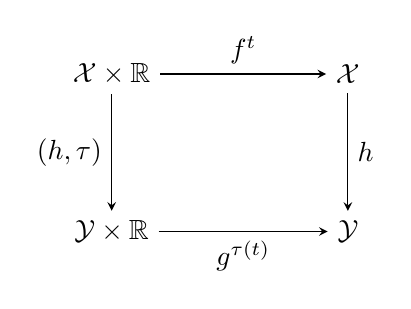
\begin{tikzpicture}[>=stealth, every node/.style={draw=none}]
  % Nodes
  \node (X1) at (0, 2) {$\mathcal{X} \times \mathbb{R}$};
  \node (X2) at (3, 2) {$\mathcal{X}$};
  \node (Y1) at (0, 0) {$\mathcal{Y} \times \mathbb{R}$};
  \node (Y2) at (3, 0) {$\mathcal{Y}$};

  % Arrows
  \draw[->] (X1) -- node[above] {$f^t$} (X2);
  \draw[->] (X1) -- node[left] {$(h,\tau)$} (Y1);
  \draw[->] (X2) -- node[right] {$h$} (Y2);
  \draw[->] (Y1) -- node[below] {$g^{\tau(t)}$} (Y2);
\end{tikzpicture}
\end{center}
Having this foundation allows us to describe the geometry of the dynamical system more precisely. First, we shall see that the dynamical system has a very particular local structure around stationary points. Stationary points serve a parallel purpose to those defined in introductory calculus. For us, we will understand them as follows:
\begin{mydefinition}{Stationary Points}
Let $F:\mathcal{X}\to \mR^d$ be a $C^1$ vector field with $\mathcal{X}\subset \mR^d$ open. We say that
\begin{itemize}
	\item $p\in \mathcal{X}$ is \emph{stationary} if $F(p)=0$,
	\item a stationary point $p\in \mathcal{X}$ is \emph{simple} if the Jacobian $DF(p)$ has full rank,
	\item a simple stationary point $p\in \mathcal{X}$ is \emph{hyperbolic} if all the eigenvalues of $DF(p)$ have non-zero real parts,
	\item a hyperbolic stationary point is an \emph{attractor} if all eigenvalues of $DF(p)$ have negative real parts,
	\item a hyperbolic stationary point is a \emph{repeller} if all eigenvalues of $DF(p)$ have positive real parts, and
	\item a hyperbolic stationary point is a \emph{saddle point} if it is neither an attractor nor a repeller.	
\end{itemize}
\end{mydefinition}
It is straightforward to see that if $p$ is a stationary point of a $C^1$ vector field, then $p$ is a fixed point of the time $t$-maps of the dynamical system arising from the autonomous differential equation \ref{diffeqvf}, i.e., $f^t(p)=p$. Moreover, it is not too hard to show that $Df_p(t)=\exp(tDF(p))$ with $f_p$ the trajectory of $p$. This allows us to translate the properties of the vector field into properties in terms of the flow. With this terminology settled, we will look at how these definitions correspond to the geometric properties of flows around stationary points. One classical result is the Grobman-Hartman theorem:
\begin{thm}[Grobman-Hartman Theorem for Flows]
Let $p\in \mathcal{X}$ be a hyperbolic stationary point of a $C^1$ vector field $F:\mathcal{X}\to\mR^d$. Then there exist neighborhoods $\mathcal{V}$ of $p$ and $\mathcal{W}$ of $0\in \mR^d$, and a topological conjugacy $H:\mathcal{V}\to\mathcal{W}$ with $H(p)=0$ conjugating the flow of $F$ restricted to $\mathcal{V}$ to the flow of the linear vector field $x\mapsto DF(p)x$ restricted to $\mathcal{W}$.
\end{thm}
This theorem shows that we can linearize the flow around stationary points, which, in turn, gives way to a much richer description of the geometry of the flow. We find that we can aptly describe this structure with the theory of manifolds. The key reasoning behind this result is that we can extrapolate behavior around the fixed points of a flow from the linearization given by the Grobman-Hartman Theorem. We record all this structure in the following result, which is also the main result of this theoretical section. It links the theory of dynamical systems with the theoretical results on state space reconstruction, which we will consider in the rest of the chapter through the introduction of manifolds. It goes as follows:
\begin{thm}[Stable Manifold Theorem]\label{stable}
Let $F:\mathcal{X}\to \mR^d$ be a $C^k$ vector field, $k\geqslant 1$, at let $p\in \mathcal{X}$ be a hyperbolic stationary point, and let $A:\mR^d\to\mR^d$ be the linear map $x\mapsto DF(p)x$. Moreover, let $(f^t)_t$ be the flow of $F$. Then there exists invariant subspaces $E^s,E^u\subset\mR^d$, satisfying that 
\begin{enumerate}[label=(\roman*)]
	\item $E^s,E^u$ decompose $\mR^d$: $\mR^d=E^s\oplus E^u$,
	\item $E^s,E^u$ are invariant under $A$: $A(E^s)\subset E^s$ and $A(E^u)\subset E^u$,
	\item all eigenvalues of a matrix representing $A|_{E^s}$ have negative real parts, and all eigenvalues of a matrix representing $A|_{E^u}$ have positive real parts.
\end{enumerate}
Moreover there exist injective $C^k$ maps $\psi^s: E^s\to \mathcal{X}$ and $\psi^u:E^u\to\mathcal{X}$ satisfying that
\begin{enumerate}[label=(\roman*)]
\setcounter{enumi}{3}
	\item $\psi^s(0)=\psi^u(0)=p$,
	\item $D\psi^s(0)E^s=E^s$ and  $D\psi^u(0)E^u=E^u$,
 \item $\psi^s,\psi^u$ are of maximal rank: for all $u\in E^s$, $$\rank D\psi^s(u)=\dim E^s$$ and for all $v\in E^u$, $$\rank D\psi^u(v)=\dim E^u,$$
 \item and the images of $E^s$ (resp. $E^u$) under $\psi^s$ (resp. $\psi^u$) are attracting (resp. repelling):
 \begin{align*}
  \psi^s(E^s)&=\{x\in \mathcal{X}:\lim_{t\to\infty}f^t(x)=p\},\\
 \psi^u(E^u)&=\{x\in \mathcal{X}:\lim_{t\to\infty}f^{-t}(x)=p\}
 \end{align*}
\end{enumerate}
\end{thm}
This theorem implies that if we have reason to believe that we are observing trajectories from a dynamical system that converges to some steady state or limit, then the theorem above realizes that trajectory on a suitable set with a lot of structure. We will quickly see that these sets are manifolds and thus serve as motivation for the notation-heavy introduction to manifolds. As for the proofs of the Grobman-Hartman theorem and the stable manifold theorem, we refer once more to \cite{Dynamics}. Before that, there are several essential remarks to make to this theorem:
\begin{itemize}
	\item If $p$ is an attractor, then we see that $E^s$ is all of $\mR^d$, and if $p$ is a repeller, then $E^u$ is all of $\mR^d$. In particular, if $p$ is an attractor, we observe by the mere fact that $\mathcal{X}\subset \mR$ that the attractor set $\psi^s(E^s)$ is a neighborhood of $p$, so everything around $p$ will converge to this point. 
	\item If $\mathcal{X}$ is compact and convex, then it is a consequence of Brouwer's fixed point theorem that a time $t$-map $f:\mathcal{X}\to\mathcal{X}$ has a fixed point $p\in \mathcal{X}$, and if it is hyperbolic this activates the stable manifold theorem. This is, in fact, a stronger statement than that of the stable manifold theorem since it implies the latter by the correspondence between fixed points of time $t$-maps of a vector field and stationary points of the vector field.
	\item It is a generic property that a linear map $\mR^d\to\mR^d$ is hyperbolic, meaning that the set of hyperbolic linear vector fields is an open and dense subset of the space of linear maps $\mathcal{L}(\mR^d,\mR^d)$ equipped with a norm; when fixing a basis we can represent all linear maps with a matrix, and induce a norm as the usual norm on $\mR^{d^2}$ of the vectorized matrix.
\end{itemize}
We see that the stable manifold theorem can be more eloquently formulated in the language of manifolds. In practice, the manifolds we will consider can always be thought of as subspaces of $\mR^d$ for a suitable dimension $d\in \mN$. However, it helps maintain some notational simplicity, and not much intuition is lost. To that end, we do some heavy lifting now in generalizing the basic concepts from calculus to the world of differential topology and manifolds in order to formulate the theorems in subsequent sections better:
\begin{mydefinition}{Manifolds}
Let $M$ be a separable Hausdorff space and let $m\in \mN$.\\[5pt]
We call $(U,h)$ a \emph{chart} if $U\subset M$ is open and $h: U\to \mR^m$ is a homeomorphism onto its range with $U$ the \emph{chart domain} and $h$ the \emph{coordinate function}.\\[5pt]
If for each point $x\in M$, there exists a chart $(U,h)$ on $M$ such that $x\in U$, we call $M$ a \emph{manifold of dimension $m$}, and we call a collection of charts whose chart domains cover all of $M$ an \emph{atlas}. The collection of all charts on $M$ is itself an atlas that we call the \emph{structure} on $M$.\\[5pt]
On overlapping chart domains of charts $(U,h)$ and $(V,g)$, we consider the \emph{coordinate transformations}
$$hg^{-1}: g(U\cap V)\to \mR^m, \text{ and } gh^{-1}: h(U\cap V)\to \mR^m$$
We say that $M$ is \emph{differentiable} if $hg^{-1}, gh^{-1}$ are differentiable for all charts, we say the charts are \emph{$C^r$-related} if the coordinate transformations $hg^{-1}, gh^{-1}$ are $C^r$, and if all coordinate transformations of an atlas are $C^r$-related, we say the atlas is \emph{$C^r$-differentiable}. A \emph{differential structure} is the set of all charts $C^r$-related to the charts in some atlas. We shall say a manifold is $C^r$ if there exists a $C^r$-differentiable atlas of $M$.\\[5pt]
If $M$ is $C^r$ and $N$ is a $C^r$ manifold of dimension $n\geqslant m$, the function $f: M\to N$ is \emph{$C^r$-differentiable} if for each $p\in M$, there exists charts $(U,h)$ on M and $(V,g)$ on N, such that $p\in U$, $f(p)\in V$ and 
$$gfh^{-1}: h(U\cap f^{-1}(V))\to \mR^n$$
is $C^r$. We then write $f\in C^r(M,N)$. (Remark: this property thus holds for any choice of charts in the atlas covering $p$ and $f(p)$ respectively). The \emph{Jacobian} at $p$ is then defined as 
$$Dgfh^{-1}(h(p))$$
This depends on the choice of charts, but the rank does not.\\[5pt]
If the Jacobian is of maximal rank (rank $m$), we say $f$ is \emph{immersive at p}, and if $f$ is immersive everywhere, then we say $f$ is an \emph{immersion}. An immersion that is homeomorphic upon its image is an \emph{embedding}.\\[5pt]
Conversely, if $m\geqslant n$, and the Jacobian is of maximal rank (rank $n$), then $f$ is \emph{submersive at $p$}, and if submersive everywhere it is a \emph{submersion}. If $f: M\to N$ is an embedding, we say that $f(M)$ is a \emph{submanifold} of $N$.\\[5pt]
A \emph{diffeomorphism} is a map $f:M\to N$ for which a differentiable inverse exists; in this case, we shall call $M$ and $N$ \emph{diffeomorphic}. If both $f$ and its inverse are $r$ times differentiable, we say $f$ is a \emph{$C^r$ diffeomorphism}, we will then write $f\in \text{Diff}^r(M,N)$, and if $M=N$, we write $f\in \text{Diff}^r(M)$. If $f$ is an embedding, it is possible to prove that $f:M\to f(M)$ is a diffeomorphism.\\[5pt]
The \emph{tangent space} to a differentiable manifold $M$ at the point $p\in M$ is the set, denoted $T_pM$, of the equivalence classes under the equivalence relation defined as follows: Let $\mathcal{C}(p)$ be the set of curves $c:I\to M$, $I\subset \mR$ an open set with $0\in I$, differentiable at $0$ and satisfying $c(0)=p$. We let $c_1\sim c_2$, if there exists a chart $(U,h)$ with $p\in U$ on $M$ such that $(h\circ c_1)'(0)=(h\circ c_2)'(0)$. We have the following local characterization on the chart $(U,h)$:
$$Dh(p):T_pM\to\mR^d,\quad [c]\mapsto (h\circ c)'(0)$$
\end{mydefinition}
\noindent We recognize immediately that the maps $\psi^s$ and $\psi^u$ of the stable manifold theorem (Theorem \ref{stable}) are injective $C^k$ immersions, and that the attractor and repeller sets $W^s(p)\coloneqq \psi^s(E^s)$ and $W^u(p)\coloneqq \psi^u(E^u)$ are indeed manifolds, that we usually call respectively the \emph{stable manifold} and the \emph{unstable manifold}. With this theorem, we also obtain a description of what happens when moving towards an equilibrium of a system. We end this section by extending the theory of dynamical systems to this manifold setting, which allows for a straightforward extension of our causal models. However, we will not make it explicit here. 
\begin{mydefinition}{Differential Equations on Manifolds}
A \emph{vector field} on a manifold $M$ is a map $F:M\to TM=\bigcup_{p\in M}T_pM$ with $F(p)\in T_p$, and a \emph{differential equation} on $M$ is given by
\begin{equation}\label{diffeqmanif}
x'(t)=F(x(t))
\end{equation}
meaning that for a chart $(U,h)$ on $M$, then
$$\forall x(t)\in U: (h\circ x)'(t)=Dh(F(x(t)))$$
with $x:\mR\to M$ a differentiable curve on $M$.
\end{mydefinition}
We solve differential equations on manifolds by localization on charts, using the results from Theorem \ref{ThmDiffEq} to generate solutions. Of course, some technicalities arise in this context, but it is mainly a matter of looking at the behavior on overlapping charts and using the properties of the coordinate transformations. In all essence, we can give the following analogy of Theorem \ref{ThmDiffEq}:
\begin{thm}[Solutions to Differential Equations on Manifolds]\label{ThmManifDiffEq}
Let $M$ be a $C^1$-manifold of dimension $d$, and let $F:M\to TM$ be a $C^1$ vector field. Then
\begin{enumerate}[label=(\roman*)]
	\item for every $p\in M$, there exists a solution $x:I\to M$ to the equation \ref{diffeqmanif} with $0\in I$ and $x(0)=p$.
	\item if $x_1:I_1\to M$ and $x_2:I_2\to M$ are solutions to the equation \ref{diffeqmanif} with $0\in I_1\cap I_2$ and $x_1(0)=x_2(0)$, then $x_1(t)=x_2(t)$ for all $t\in I_1\cap I_2$.
	\item The differential equation \ref{diffeqmanif} defines the flow $(f^t)_t$ with $f^t(p)=x(t)$ for all $p\in M$ and $x$ the unique solution going through $p$ at $0$.
\end{enumerate}

\end{thm}
\section{Takens' Theorem}
We now have the machinery to take on Takens' theorem. We have abstracted away the differential equations from previous chapters not for needless abstraction but because the theory we shall be exploiting holds and is formulated in this generality. Moreover, Takens' theorem, in its first and simplest version, holds for compact smooth manifolds. The connection with the DCMs is flimsy since most DCMs do not entail nice compact smooth manifolds. However, we have seen that manifolds do arise from dynamical systems via the stable manifold theorem. We do not use the terminology \enquote{smooth} as a precise term; it generally means that the manifold is $C^r$ for high enough $r$ to establish the result in question. If we want to ensure that the flow does live on a compact manifold, we will have to use the general construction of differential equations on manifolds, which are much less intuitive.\\\\
Why then concern ourselves with Takens' theorem? For one thing, it is a relatively compact theorem, providing a strong result in this setting. It helps illustrate the methodology, and then we can generalize sufficiently later in this chapter to capture phenomena more likely to arise from DCMs or at least a wider range of phenomena. Another note is that as long as we consider compact manifolds, we might as well envision our models living in a usual Euclidean space $\mR^n$ - Takens' theorem itself provides a proof of this fact. It is, however, not of any use when stating or proving the results, and we will, therefore, not make further reference to it. The fundamental result we shall use, now known as Takens' theorem, was proved in 1981 by Floris Takens, \cite{Takens}, and states that one can reconstruct a compact manifold using only a univariate observation function, that is observing only one variable over time allows us to reconstruct the state space of the dynamical system of all variables. The original theorem, as stated by Takens, is as follows:
\begin{thm}[Takens' Theorem, Version 1]
Let M be a compact $C^2$ manifold of dimension $m$. For pairs $(\varphi,y)\in \text{Diff}^2(M)\times C^2(M,\mathbb{R})$, it is a generic property that the map $\Phi_{(\varphi,y)}:M\to \mathbb{R}^{2m+1}$, defined by
$$\Phi_{(\varphi,y)}(x)=(y(x),y(\varphi(x)),...,y(\varphi^{2m}(x))),$$
is an embedding. \cite{Takens}
\end{thm}
There are several things to unpack here. First, it is worth noting the differentiability constraints on our maps; both $\varphi: M\to M$ and $y:M\to\mR$ must be twice continuously differentiable. In the work of \cite{Sauer1991}, their setup enables this requirement to be relaxed to them only being once continuously differentiable - we will cover that shortly. Next, we will call $y$ our \textit{observation function} as introduced at the beginning of the chapter. We can think of this as what we observe from the system, and it will replace random variables in this dynamical systems setting. The background space is now a dynamical system instead of a probability space, and the measurability of a random variable translates to the differentiability of an observation function. For now, $\varphi$ is defined very generally, but we shall quickly make this map much more explicit as a time $t$-map.\\\\
We shall call $\Phi$ the \textit{delay embedding}, the reasoning behind which will be revealed shortly. However, the most important caveat is perhaps that it is \enquote{only} a generic property that the theorem yields a reconstruction of the manifold, i.e., that the delay embedding is an embedding. By generic property, it is meant to be understood that the delay embedding is indeed an embedding for \enquote{most} observation functions $y$ and \enquote{most} choices $\varphi$. So, this concept takes the place of \enquote{almost surely} from probability theory. The precise meaning in an algebraic sense is that there exists an open and dense subset of the function space $C^2(M,\mR)$, respectively $\text{Diff}^2$, for which the statement is true when using the following topology generated by the subbase consisting of sets defined as follows:\\[5pt]
For any choice of function $f\in C^r(M,N)$, charts $(U,h)$ on $M$ and $(V,g)$ on $N$, a compact set $K\subset U$ such that $f(K)\subset V$ and $\varepsilon>0$, we define $\mathcal{N}(f,(U,h),(V,g),K,\varepsilon)$ to be the set of all functions $\hat{f}\in C^r(M,N)$ for which $\hat{f}(K)\subset V$ and
$$\norm{D^kg\hat{f}h^{-1}(x)-D^kgfh^{-1}(x)}<\varepsilon$$
for all $x\in h(K)$, $k=0,\ldots,r$, where $\norm{\cdot}$ is the usual Euclidean norm. If $M$ and $N$ are diffeomorphic, we let $\text{Diff}^r(M,N)$ be the subspace of $C^r(M,N)$ consisting of $C^r$-differentiable diffeomorphisms equipped with the subspace topology.\\\\
From this stems our second regularity assumption. For $\varphi$, we can do some reasoning in practical cases, but for $y$, this will often be just another silent assumption. We shall be calling a map $y\in C^2(M,\mR)$, respectively $\varphi\in \text{Diff}^2(M)$, \textit{generic} if there exists $\varphi\in \text{Diff}^2(M)$, respectively $y\in C^2(M,\mR)$, such that the resulting delay embedding is indeed an embedding.
We will now work towards a more explicit version of the theorem. First of all, the reasoning behind the naming of the delay embedding comes from the following: if we imagine a $C^2$ flow $(\varphi^t)_{t\in \mR}$ on $M$, and consider a point $x\in M$, then we let $x(t)=\varphi^t(x)$ denote the location of the flow after time $t$ going through $x$ at $0$. We can think of this as the position of a given trajectory at time $t$ on the manifold. If we then fix a delay size $\tau\in \mR$ by substituting into Takens' theorem, we can reduce the delay embedding to
\begin{align*}
\Phi_{(\varphi,y)}(x(t))&=\left(y(x(t)),y(x(t-\tau)),\ldots,y(x(t-2m\tau))\right)\\
&=\left(y(\varphi^t(x)),y(\varphi^{t-\tau}(x)),\ldots,y(\varphi^{t-2m\tau}(x))\right)
\end{align*}
Takens' theorem thus states that the values of a single time series considered at different delays will reconstruct the manifold \enquote{generically}. Now, we will need to ensure that this choice of $\varphi$ is both twice continuously differentiable and is not of such a nature that it falls out of the set of generic functions. The differentiability constraint falls under the umbrella of regularity assumptions and is fulfilled for flows arising from autonomous differential equations of $C^2$ vector fields. Furthermore, we can guarantee that $\varphi^\tau$ will be generic for some choices of $\tau$ by the power of a restatement of Takens' theorem. Takens proved the result himself in \cite{Takens} but did not state it. We will follow the restatement of the theorem and the subsequent presentation of theory and definitions presented in \cite{Huke} for the rest of this section. We present the updated version of Takens' theorem:
\begin{thm}[Takens' Theorem, Version 2]\label{v2}
Let M be a compact $C^2$ manifold of dimension $m$. Let $\varphi\in\text{Diff}^2(M)$ satisfy
\begin{enumerate}[label=\arabic*)]
	\item the periodic points of $\varphi$ with periods less than or equal to $2m+1$ are finite in number,
	\item if $x$ is any such periodic point with period $p\leqslant 2m$, then the eigenvalues of $\varphi^k$ at $x$ are all distinct.
\end{enumerate}
 Then it is a generic property for $y\in C^2(M,\mR)$ that the map $\Phi_{(\varphi,y,k)}:M\to \mathbb{R}^{2m+1}$, defined by
\begin{equation}\label{delayemb}
\Phi_{(\varphi,y,k)}(x)=(y(x),y(\varphi(x)),...,y(\varphi^{k}(x))),
\end{equation}
is an embedding for $k\geqslant 2m$. \cite{Huke}
\end{thm}

By periodic with a period less than or equal to $2m$, we mean that $\varphi^{p}(x)=x$ for some $p\leqslant 2m$. The proof of the theorem is quite involved, and a thorough treatment of the technicalities and details is perhaps worthy of a thesis of its own. We will still outline the proof to illuminate the machinery of this theory. In the following, we will use the subspace topology on $C^2(M,\mR)$ inherited from $C^1(M,\mR)$ and likewise on $\text{Diff}^2(M)$. In all topological statements below, this is what is meant. The proof of the 2nd version of Takens' theorem runs in the following stages:
\begin{enumerate}[label=\roman*)]
	\item First, we prove that the set of generic observation functions is open, and we basically just exploit the following standard fact in differential topology:
	\begin{thm}\label{tool}
	Let $M$ be a compact manifold and $N$ be any manifold. For $K\subset M$ a compact subset of $M$, the set of $C^r$ maps from $M$ to $N$ immersive on $K$ is open in $C^r(M,N)$. Moreover, the set of $C^r$ embeddings of $M$ in $N$ is open in $C^r(M,N)$. \cite{hirsch}
	\end{thm}
	Proving that the map $\mathcal{F}^2: C^2(M,\mR)\to C^2(M,\mR^{2m+1})$, defined by $$y\mapsto (y,y\circ\varphi,\ldots, y\circ \varphi^{2m}),$$ 
	is continuous, then immediately proves that the set of generic observation functions is open in $C^2(M,\mR)$. This is done in the following familiar set of steps: one proves $F: C^2(M,\mR)\to C^2(M,\mR)$ defined by $y\mapsto y\circ\varphi$, for $\varphi\in \text{Diff}^2(M)$, is continuous. This is simply a matter of unraveling the definition of the topology above and requires only a slight bit of trickery. We skip the details of these derivations. By induction, it follows that $F_n:  C^2(M,\mR)\to C^2(M,\mR)$ defined by $y\mapsto y\circ\varphi^n$ is in fact continuous.  The final detail is to use that the product topology of $C^r(M,\mR)^{2m+1}$ coincides with that of $C^r(M,\mR^{2m+1})$. Worth remarking here is that we have made no assumptions on $\varphi$ yet; any embedding will do. Likewise, we have yet to use $m$ for anything. 
\end{enumerate}
The rest of the stages are about proving that the set of generic observation functions is also dense. We start this process by picking any observation function $y$ and any neighborhood $\mathcal{N}$ of our observation function. We then proceed to locate a generic observation function within this neighborhood by iteratively adjusting the observation function to ensure the resulting delay embedding satisfies one more criterion for an embedding. In this pursuit, we will frequently use Theorem \ref{tool} and the following technical fact: If $y\in C^2(M,\mR)$, and $\psi_i\in C^2(M,\mR)$, $i=1,\ldots,N$ for some $N\in \mN$. Then for every neighbourhood $\mathcal{N}$ of $y$, there exists $\delta$ such that
\begin{equation}\label{tool2}
\forall a=(a_1,\ldots,a_n),\norm{a}< \delta: y+\sum_{i=1}^N a_i\psi_i\in \mathcal{N}
\end{equation}
Proving this is only a matter of exploiting the compactness of $M$ and using the definition of the topology on our function space. We proceed as follows:
\begin{enumerate}[label=\roman*)]
	\setcounter{enumi}{1}
	\item The next step is locating an immersion on the set of points with a period less than or equal to $2m$; let us denote it $P_{2m}$. In this stage, we use our assumptions on $P_{2m}$: Since $|P_{2m}|<\infty$, we know by the Hausdorff property of $M$, that we can find pairwise disjoint neighborhoods of the elements in $P_{2m}$, and thus separate the different elements of $2m$. Now, by a fairly standard construction, we can, for any point and two nested neighborhoods of it, assume the existence of a \enquote{bump function}, i.e., a $C^2$ function taking a positive value in the point, having derivative 0 in the smaller neighborhood and being 0 outside the larger neighborhood. This allows us to manipulate each of these points separately. Using that the eigenvalues of $\varphi^k$ at each point are all distinct, we can manipulate the Jacobian of $\Phi_{\varphi,y}$ using the chain rule and pushing $y$ around with \ref{tool2} to ensure that it gets full rank. The considerations in \ref{tool2} allow us to do this iteratively. If we find an immersion $y'$ of some subset $A\subset P_{2m}$, then we can find a neighborhood contained in $\mathcal{N}$ containing $y'$ where all elements are immersions of $A$. This is true by theorem \ref{tool} and stage i) since the set of such immersions is open. After carefully handling this manipulation in each step, we can guarantee the existence of an immersion $y'$ on $P_{2m}$ inside $\mathcal{N}$.
	\item The next stage is to extend this procedure to an immersion on all of $M$. In this stage, we use the dimension of $m$: First, we note that by the inverse function theorem, $y'$ is an embedding of a neighborhood of each point $p\in P_{2m}$ and thus an immersion of that neighborhood. We then proceed to cover $M$ with charts:  We choose charts containing an element $p\in P_{2m}$ small enough to ensure that $y'$ is an immersion of its closure, and for an element $p\notin P_{2m}$, we have $p,\varphi(p),\ldots, \varphi^{2m}(p)$ are distinct. Thus we can choose a chart $U_p$ of $p$ such that $U_p,\varphi(U_p),\ldots, \varphi^{2m}(U_p)$ are disjoint. Furthermore, in each set, we move to a smaller chart whose closure is contained in the larger chart. By compactness of $M$, this cover can be thinned to a finite number of charts. In this stage, our map is then iteratively extended to an immersion on the closure of a chart not immersed already. Using a bump function on each chart and its image under $\varphi,\ldots,\varphi^k$ allows us once again to manipulate the Jacobian of $\Phi_{(\varphi,y)}$ by allowing us to push each coordinate separately using \ref{tool2}. Using a standard argument, we can show that if the $s+1$'th column of the Jacobian is not linearly independent of the first $s$ linearly independent columns at any element of the chart, then this parametrizes a subspace of dimension $s+m$ of $\mR^{2m+1}$ for values of $a$. The complement of this subspace is naturally open and dense; thus, we can find an element of any norm for which all columns are independent. This argument is, in fact, valid for only $2m$ coordinates of $\Phi$; we need $2m+1$ to establish injectivity later on. Nonetheless, this identifies a perturbed observation function immersive on the closure of the entire chart - and by Theorem \ref{tool} and stage i), this can be done iteratively to find $y''\in \mathcal{N}$ immersive on all of $M$.
	\item The final stage of the proof of the 2nd version is to establish injectivity. By the Inverse Function Theorem, this is true locally, so we will try to extend this local property to a global. This stage is by far the most technical part of the proof. Proving that there exists $y'''\in \mathcal{N}$ such that $\Phi_{(\varphi, y''')}(x)\neq \Phi_{(\varphi, y''')}(\varphi^j(x))$ unless $x=\varphi^j(x)$ can be achieved with a similar construction as in iii) separating charts, on which $\Phi_{(\varphi,y'')}$ is an embedding, such that the images under $\varphi^j$, $j=0,\ldots,m$, are disjoint and then thinning to a finite number of charts before adjusting. Since $\Phi_{(\varphi,y''')}$ is injective in small neighbourhoods around all points in $M$, we then have for any $x,x'\in M$, $x\neq x'$, that if $\varphi^i(x)$ and $\varphi^j(x)$ land in the same small neighbourhood for say $i,j\leqslant 2m$, then $\Phi_{(\varphi,y''')}(x)\neq \Phi _{(\varphi,y''')}(x')$. Thus, separating orbits close to each other allows us to look at the subset of $M\times M$ where this phenomenon does not happen. Identifying once more a reasonable cover of charts of $M$ well-behaved under $\varphi$, one can choose a partition of unity subordinate to this cover, that is, a map for each chart that is zero outside the chart such that the sum of all functions in each point is 1. Looking then at \ref{tool2} where we name the element $y_{\varepsilon}$ of the perturbation of $y'''$ with the $\psi$-functions the partitions of unity and coefficients $\varepsilon_1,\ldots,\varepsilon_N$. We need to show that these coefficients can be chosen such that $\Phi$ becomes injective while still being sufficiently small. This is done by checking the image of $\Psi:M\times M\times \mR^N\to\mR^{2m+1}$ given by
	$$\Psi(x,x',\varepsilon_1,\ldots,\varepsilon_N)=\Phi_{(\varphi,y_{\varepsilon}})(x)-\Phi_{(\varphi,y_{\varepsilon}})(x')$$
	We will not spend more time on this part of the proof, but this is the part where it becomes crucial to go to $\mR^{2m+1}$ and not $\mR^{2m}$ since the dimension of the domain of $\Psi$ is $2m+N$, and we need $\Psi|_{X}^{-1}(0)$ to be of lower dimension than $N$. This allows us to choose $\varepsilon$'s to satisfy the constraint and yield an embedding. 
	\item The final stage is proving the 1st version of Takens' theorem from the 2nd version. It relies almost entirely on the Kupka-Smale theorem:
	\begin{thm}[Kupka-Smale Theorem]
	If $M$ is a compact manifold, and $\varphi\in \text{Diff}^2(M)$, then it is a generic property that for some integer $n\in \mN$, that the number of periodic points with period $n$ or less is finite.
	\end{thm}
	There is a little work in showing that one can extend this when incorporating the second condition of the second version of Takens' theorem. One also needs to use an argument similar to that in stage i) to prove the openness claim in the function space $\text{Diff}^2(M)\times C^2(M,\mR)$ instead of just in $C^2(M,\mR)$. However, in essence, the Kupka-Smale theorem is the link between the two theorems.
\end{enumerate}  
The theorem warrants a few comments. First, we need to deal with periodic points quite explicitly. If we do not expect periodic points of the flows we observe, then Takens' theorem greatly simplifies. Moreover, when working with flows, the time lag could be varied a bit to yield a generic function. More theory is needed to handle this explicitly, but in principle, multiple lags could be tested in practice, and in this case, we should be able to sidestep this problem. Often, we will assume that we have a nice time lag, and Takens' theorem guarantees that it is a generic property. \\[5pt]
In contrast to the choice of delay size $\tau$ when formulating the delay embedding, we will generally have less flexibility in the choice of observation functions. So, even if the same technique of small perturbations of a non-generic observation function produces a generic observation, we do not have access to it. Therefore, we will usually assume a given observation function is generic if there is no reason to believe otherwise. Takens' theorem gives us confidence that this can be assumed since it is a generic property. However, in some cases, we can actually endow genericity with causal interpretation - we return to this in the next section.\\[5pt]
Even though Takens' theorem itself appears somewhat magical, it should not be seen as too big of a surprise. As noted above, a generic property is analogous to an identity holding almost surely in probability theory, and we will also interpret them similarly. One thing holding us back from going straight into a measure-theoretic formulation is that the space of all differentiable functions is usually infinite-dimensional. So, generalizing the Lebesgue measure to such a space is not straightforward. However, it is possible to link the two concepts. To this end, we introduce the concept of prevalence:
\begin{mydefinition}{Prevalence}
Let $V$ be a normed vector space over $\mR$.\\[5pt]
The $\sigma$-algebra $\mathcal{B}$ generated by all open sets in $V$ is called the \emph{Borel $\sigma$-algebra on V} and $S\in \mathcal{B}$ is called a \emph{Borel subset of $V$}. If $V$ is finite-dimensional of dimension $d$, $V\cong \mR^d$ in the sense of isometry and this map defines a (unique) Lebesgue measure $\lambda $ on $V$.\\[5pt]
We say that a Borel subset $S\subset V$ is \emph{prevalent} if there is a finite-dimensional subspace $E$ of $V$ such that for each $v\in V$, we have $v+e\in S$ for Lebesgue almost every $e\in E$, i.e.
$$\lambda_E\left(\left\{e\in E\mid v+e\notin S\right\}\right)=0$$
We then call $E$ a \emph{probe space of $S$}.\\[5pt]
If $S$ is a prevalent subset of $V$, then we say that $v\in S$ for \emph{almost every $v\in V$}.
\end{mydefinition}
We see that a prevalent set satisfies that if we start at any point in the ambient space $V$, then any exploration according to the directions of the finite-dimensional probe space will end in $S$ almost surely. This captures the essence of $S$ inhabiting \enquote{most of} $V$ in the \enquote{directions of $E$}. This becomes immediately more appealing once we realize this is much more all-encompassing than it seems at first glance: Assume that $E'\subset V$ is a finite-dimensional subspace containing a probe space $E$ of $V$. Let $v_1,\ldots,v_n$ be an orthonormal basis of $E'$, such that $v_1,\ldots,v_k$, $k<n$, spans $E$. By Fubini's theorem, we then realize
\begin{align*}
\lambda_{E'}\left(\left\{e'\in E':v+e\not\in S\right\}\right)&=\int 1_{\{e'\in E'\mid v\in e'\notin S\}}\ d\lambda_{E'}\\
&=\int\int 1_{\{e'\in E'\mid  v\in e'\notin S\}}\ d\lambda_{E}\ d\lambda_{\langle v_{k+1},\ldots, v_n \rangle}\\
&=0
\end{align*}
This means we can arbitrarily extend a probe space, so $S$ is really \enquote{everywhere} in $V$ if $S$ is prevalent. This motivates the definition of \enquote{almost every} as an extension of almost surely. Indeed, when $V$ is finite-dimensional, we recognize that the complement of a prevalent set has Lebesgue measure 0. This concept of prevalence is not one-to-one with the concept of genericity but allows for similar embedding theorems. Quite importantly, we can formulate Takens' theorem with this concept instead:
\begin{thm}[Takens' Theorem, Version 3]
Let M be a compact $C^1$ manifold of dimension $m$. Let $\varphi\in\text{Diff}^1(M)$ satisfy
\begin{enumerate}[label=\arabic*)]
	\item the periodic points of $\varphi$ with periods less than or equal to $2m+1$ are finite in number,
	\item if $x$ is any such periodic point with period $k\leqslant 2m$, then the eigenvalues of $\varphi^k$ at $x$ are all distinct.
\end{enumerate}
 Then for almost every $y\in C^1(M,\mR)$, the map $\Phi_{(\varphi,y)}:M\to \mathbb{R}^{2m+1}$ defined by
$$\Phi_{(\varphi,y)}(x)=(y(x),y(\varphi(x)),...,y(\varphi^{2m}(x))),$$
is an embedding. \cite{Sauer1991}
\end{thm}
This result relaxes the $C^2$ assumption but is otherwise nearly identical to version 2. In fact, Takens' embedding theorem is only a particular result of a quite general phenomenon. This is made explicit in a result of \cite{Sauer1991}, which restates the Whitney embedding theorem in the following way:
\begin{thm}[Whitney Embedding Prevalence Theorem]
Let $M$ be a compact $C^1$ manifold of dimension $d$. Almost every $C^1$ map $M\to \mR^{2d+1}$ is an embedding of $M$.
\end{thm}
This shows that, in reality, it is more a feature of manifolds than any particular feature of the delay embedding that allows us to reconstruct a manifold. The relevance of Takens' theorem thus stems more from its practicality than its theoretical implications on the existence of embeddings. When working with time series, the delay map is a very natural construction, and Takens' theorem gives theoretical backing to its usability. 

\section{Causal Inference with Takens' Theorem}
We are now ready to formulate identifiability results for dynamical systems. The results of this section are lifted straight from \cite{mathFound}, but we choose to formulate them in slightly different terms. First of all, as already discussed, we follow their terminology on fully resolved state spaces with a subtle deviation, and therefore, we incur some changes in formulations further on. In this section, we chose to present results in a relatively simple setting as illustrations of the causal discovery techniques of dynamical systems to build some intuition rather than as directly applicable results to DCMs. This choice manifests itself in several ways: All results in this section assume state spaces are compact manifolds, even though that may not be the most natural when considering real-world examples. We shall later provide more general results, but it allows for more accessible results. Also, there are some technical results in this setting that we do not have in the more general setting.\\\\
Moreover, we choose to present results highlighting how delay embeddings can reveal some of the graphical structure, and not as in \cite{mathFound} as results establishing a complete characterization of the graphical structure that can be identified. In all essence, there is no difference in the theoretical contents of the two presentations. However, we prefer to formulate it to show the implications of Takens' theorem if only two state spaces are sufficiently well-behaved. We will comment on these differences again when we have formulated our results.\\\\
We have covered how the graphical structure can be represented in dynamical systems, and we have established how we generically can reconstruct state spaces via a delay embedding involving only a single variable if the state space is a compact smooth manifold. Combining these two ideas, we get to the central idea of the causal inference mechanisms of this thesis. If we can reconstruct the state space and infer properties of the graphical structure from this, we can then infer information about the causal structure. The graphical structure is represented via a filtration and the Takens property, and the missing ingredient is then the question of whether Takens' theorem holds for the sub-state spaces. First, we have to assume that the assumptions on the state space are once again fulfilled. Continuous mappings preserve compactness, so there is no problem with that assumption, but the manifold structure is not generally preserved. For instance, there does not exist a compact smooth manifold in $\mR$ as we have defined them because it would be a closed and bounded set, and therefore, there exists a maximal element on which it is possible to locate a chart. This means that when using flows from DCMs, we will always encounter problems for variables with no parents. Accepting that we cannot establish this property as a general property, we will instead assume it away for now, but note that we can do more when moving to a more flexible framework in the next section.\\\\
If we now, for a moment, assume that our state spaces are compact manifolds, the next question is whether it is still a generic property that each subflow of a flow satisfying the Takens property is generic. More precisely, we want to prove that the conditions of Theorem \ref{v2} are fulfilled for each subflow. We give the following result of \cite{mathFound} establishing this in general:
\begin{thm}[Genericity over Filtrations]\label{tech}
Let $M$ be a compact $C^2$ manifold $M$ of dimension $m$ admitting a filtration $(M_U,\pi_{UV})_{\an(\mathcal{G})}$ with respect to a chain graph $\mathcal{G}$. Let $\mathcal{U}\subset \an(\mathcal{G})$ be a subset for which $M_U$ is a $C^2$ manifold of dimension $m_U$ for all $U\in \mathcal{U}$. It is then a generic property for $\varphi\in C^2(M,M)$ satisfying the Takens property that for each $U\in \mathcal{U}$: 
\begin{enumerate}[label=\arabic*)]
	\item the periodic points of $\varphi_U$ with periods less than or equal to $2m_U+1$ are finite in number,
	\item if $x$ is any such periodic point with period $k\leqslant 2m$, then the eigenvalues of $\varphi^k_U$ at $x$ are all distinct.
\end{enumerate}
\end{thm}
The proof of this fact is very technical and would take up significant space. We refer to the proof of \cite{mathFound} and use the result as a marker that generic properties are well-behaved across this type of construction. Moreover, it is quite practical that we do not have to make assumptions on this part. We do not know if such a result can be established when moving to a more general setting. This theorem, combined with Takens' theorem (Theorem \ref{v2}), yields that it is a generic property for observation functions to give us an embedding of the manifold $M_U$. This allows us to formulate the main theorem in the manifold setting, the proof of which is now deceptively simple because of the substantial set of assumptions we have built up. We make one final observation before giving the theorem:\\[5pt]
In the theorem, we will talk about observation functions on a submanifold $M_U$ obtained from the filtration of the state space $M$. Notice, however, that thanks to the filtration of the state space, this defines an observation function $y_1\circ\pi_U:M\to \mR$ on $M$. We can, therefore, think of an observation function $y$ as living both on the whole state space and on $M_U$ if it decomposes to $y_U\circ \pi_{U}$ for some observation function $y_U$ on $M_U$. By the same argument, this holds true for any pair of nested ancestral sets $U\subset V$ as well, since we can define $y_V=y_U\circ \pi_{VU}:M_V\to \mR$ for $y_U:M_U\to \mR$ an observation function. This motivates the following definition:
\begin{mydefinition}{Proper Observation Functons}
Let $\mathcal{X}$ be a state space admitting a filtration $(\mathcal{X}_U, \pi_{UV})_{\an(G)}$; and let $V\in \an(G)$. We will then say that the observation function $y_V:\mathcal{X}_V\to \mR$ is \emph{proper}, if there exists no $y_U:\mathcal{X}_U\to \mR$ for an ancestral set, that is a proper subset $U\subset V$, such that $y_V=y_U\circ\pi_{VU}$, and we will say $y:\mathcal{X}\to \mR$ is \emph{proper with resepct to $V$}, if there exists a proper observation function $y_V:\mathcal{X}_V\to \mR$ such that $y=y_V\circ\pi_V$.
\end{mydefinition}
Now, we are ready to give the theorem:
\begin{thm}[Identifiability in Dynamical Systems on Manifolds]\label{id1}
Let $(\varphi,\mR,M)$ be a dynamical system, where $M$ is a compact $C^2$ manifold of dimension $m$ admitting a filtration $(M_U,\pi_{UV})_{\an(\mathcal{G})}$ fully resolving $M$, and $(\varphi_t)^t$ is a $C^2$ flow on $M$ satisfying the Takens property. Let now $U,V\in \an(\mathcal{G})$, assume $M_U$ and $M_V$ are compact $C^2$ manifolds of dimension $m_U$ and $m_V$ respectively, and assume 1) and 2) of Theorem \ref{tech} is satisfied with $\mathcal{U}=\{U,V\}$ for $\varphi^T$ for some fixed value $T\neq 0$.\\[5pt]
It is now a generic property for $C^2$ observation functions $y_1:M\to \mR$ proper with respect to $M_U$ and $y_2:M\to\mR$ proper with respect to $M_V$, that for $i=1,2$ with $k_1\geqslant 2m_U$ and $k_2\geqslant 2m_V$, we have that the delay embedding $\Phi_{(\varphi^T,y_i,k_i)}$ defined as in the expression \ref{delayemb} is an embedding of $M_U$, respectively $M_V$. Let then $$M_i=\Phi_{(\varphi^T,y_i,k_i)}(M)$$ 
be the state space reconstructions of $M_U$ and $M_V$ under the proper and generic observation functions. It holds that:
\begin{enumerate}[label=\roman*.]
	\item $U\subset V$ if and only if there exists a continuous surjective map
	$$\Pi_{2,1}:M_2\to M_1,$$ 
	\item $U=V$ if and only if there exists a homeomorphism
	$$\Psi_{1,2}:M_1\to M_2.$$
\end{enumerate}
\end{thm}
\begin{proof}
The statement on genericity of observation functions is just Theorem \ref{v2}. As for the rest, we proceed in the following steps:
\begin{enumerate}[label=\roman*.]
	\item \textit{Forward direction}: If $U\subset V$, then there exists $\pi_{VU}:M_V\to M_U$ since $M$ is fully resolved. Then
	$$\Pi_{2,1}=\Phi_{\varphi^T,y_1,k_1}^{-1}\circ\pi_{VU}\circ \Phi_{\varphi^T,y_2,k_2} $$ is a continuous surjection of $M_2$ on $M_1$.\\[5pt]
	\textit{Reverse direction}: Assume the existence of $\Pi_{2,1}$. Then
	$$\Phi_{\varphi^T,y_1,k_1}^{-1} \circ\Pi_{VU}\circ  \Phi_{\varphi^T,y_2,k_2} $$
	is a continuous surjection from $M_V$ to $M_U$. Since the manifold is fully resolved, this implies that $U\subset V$.
	\item \textit{Forward direction}: If $U=V$, then $\Psi_{1,2}=\Phi_{\varphi^T,y_2,k_2}\circ \Phi_{\varphi^T,y_1,k_1}^{-1}$ is a diffeomorphism of $M_1$ on $M_2$.\\[5pt]
	\textit{Reverse direction}: Assume the existence of $\Psi_{1,2}$. Then
	$$\Phi_{\varphi^T,y_2,k_2}^{-1}\circ \Psi_{1,2} \circ \Phi_{\varphi^T,y_1,k_1}$$
	is a homeomorphism from $M_U$ to $M_V$. By i) this implies both $U\subset V$ and $V\subset U$, and thus that $U=V$.
\end{enumerate}
\end{proof}
Now, let us make some comments on what we have achieved here. This theorem establishes that we can determine some causal directions in a dynamical system on a manifold if we can check for the existence of the maps indicated in the theorem. Let us be more precise: if there exists a partially directed path from $u$ to $v$ in the graph $\mathcal{G}$, it follows that $\an(u)\subset \an(v)$. More importantly, the converse is true, and thus, we can infer this information from the state space reconstructions by the theorem. Moreover, if the path is entirely undirected, then $\an(u)=\an(v)$, and once again, the converse is true, which makes it possible to infer from the state space reconstructions by the theorem. This also explains the use of chain graphs in this model: were we instead to have used directed graphs and allowed cycles, then the argument would go through with ancestral sets all the same. However, any ancestral set containing one vertex in the cycle would contain them all - and these components would thus be inseparable in any case. It is debatable whether the approach in this thesis is a better choice compared to this. However, at least the graph structure directly encaptures two kinds of relationships between variables.\\\\
There are limits to what we can recover with this approach. Imagine we have the following causal chain:
$$X\rightarrow Y\rightarrow Z$$
What we can recover from the theorem is then that $\an(X)\subset \an(Y)\subset \an(Z)$, and we thereby recover the causal chain, but we cannot infer whether we have a direct edge from $X$ to $Z$ besides the causal chain going through $Y$. This motivates the following definition:
\begin{mydefinition}{Transitive Closure}
Given a chain graph $\mathcal{G}=(\mathcal{V},\mathcal{E})$, the \emph{transitive  closure of $\mathcal{G}$} is the graph $\overline{\mathcal{G}}=(\mathcal{V},\overline{\mathcal{E}})$ on the same vertex set $\mathcal{V}$ obtained from $\mathcal{G}$ by keeping all existing edges and add
\begin{enumerate}[label=\roman*)]
	\item the edge $u\to v$, if there exists a partially directed path from $u\in \mathcal{V}$ to $v\in \mathcal{V}$ with at least one directed edge, and
	\item the edge $u-v$, if there exists  partially directed path from $u\in \mathcal{V}$ to $v\in \mathcal{V}$ with no directed edges.
\end{enumerate} 
\end{mydefinition}
 It is worth noting that all chain components become complete under the transitive closure, i.e., a bidirected edge exists between any pair of variables. Another way to phrase this is that a chain graph induces a preorder on the vertices, namely that $u\leqslant v$ if there exists a partially directed path from $u$ to $v$. We see that this is reflexive and transitive, and hence a preorder. Furthermore, it is antisymmetric if and only if the graph is a DAG. With this terminology in place, we can formalize our observations with the following pseudo-algorithm:
\begin{alg}
Let the set-up be as in Theorem \ref{id1}, and assume all sets $M_U$ are compact $C^2$ manifolds. This is the situation covered by \cite{mathFound} in the manifold setting. Then the following algorithm recovers the transitive closure $\overline{\mathcal{G}}$ of the graph $\mathcal{G}$:
\begin{enumerate}[label=\roman*.]
	\item Let the set of variables be the set of vertices in a graph we will call $\mathcal{G}$.
	\item For every variable $x$, build the reconstructed manifold $M_x\coloneqq \Phi	_{(\varphi^T,x,k)(M)}$.
	\item For every pair $x$ and $y$, draw an edge $x\to y$ if there exists a continuous surjection $f:M_x\to M_y$.
	\item If $x\to y$ and $y\to x$ for a pair of vertices $x,y$, then we write instead $x-y$.
\end{enumerate}
\end{alg}
The theoretical build-up to this algorithm has been quite involved, but this algorithm has an inherent simplicity compared to Granger causality. First of all, we essentially eliminate all of the assumptions (GC1)-(GC3) of Granger causality as formulated in Section \ref{multiSCM}. That we allow for deterministic relationships contrary to (GC2) is at the core of the entire theory, while the lack of separability contrary to (GC1) is a product of Takens' theorem. In this sense, the assumptions needed for this approach to be sensible are the opposite of (GC1) and (GC2). As for the final assumption on no unobserved confounders, in Granger causality, we have to account for all relevant information in order to allow for causal reasoning, whereas in this set-up, if we want to infer the causal direction between two variables, we need only consider the two time series in question. Nowhere in this algorithm do we need to observe all variables:\\[5pt]
The beauty of Takens' theorem is that if there are potential hidden or unobserved confounders, meaning that the two variables in question share a parent that we do not observe, then the dynamics of a confounder are captured within the time series that we do observe because they are further down the causal chain. An important caveat here is that we cannot rule out a causal \enquote{mirage} due to synchronization: imagine a common causal confounder between two systems resulting in two heavily synchronized, but essentially \enquote{independent} dynamical systems. Independent is, of course, not to be interpreted in the probabilistic sense but more in a causal one: interventions in one system should have no impact on the other. In the most extreme case, we could imagine two dynamical systems that are copies of one another. Then, the algorithm above would infer causal links that are not present. However, we would expect these mirages to occur only in the case of heavy synchronization, so the problem is more limited than the problem of unobserved confounders in our Granger causality framework. Moreover, in the less extreme cases, the theory should still work - and this phenomenon is essentially ruled by our assumption of a fully resolved state space.\\\\
As appealing as all of this is, we have to remark on some serious semi-practical complications of this technique as described up until this point, some of which we have already touched upon. First, it is very unrealistic to assume that the canonical filtration from a DCM induces a system of compact smooth manifolds, even if everything were to behave perfectly as described by the model. We could hope that we are somehow \enquote{close enough} for the theory to be successful either way. However, it is not especially comforting as a theoretical background when applying this theory in practice. Moreover, we assume in all our statements that we have access to the entire manifold for the state space reconstruction. However, in practice, we only have access to one single trajectory. Therefore, we cannot, in practice, reconstruct the manifold at all, which complicates applications of this section's identifiability results. We will try to address all these problems in the next section by introducing chaotic attractors, which can arise from DCMs, are preserved by the canonical filtration, and where a single trajectory can be dense in the attractor, thus allowing us to capture information on the entire state space from one observation.

\section{Chaotic Attractors}
In this section, we introduce attractors to mitigate the problems outlined at the end of the last section. The main components are thus to establish how systems of differential equations can produce attractors, establish that attractors are well-behaved against filtrations, and establish a version of Takens' theorem that can handle attractors. First up, we define attractors:
\begin{mydefinition}{Attractors}
Let $\mathcal{D}=(\varphi,\mathcal{T},\mathcal{X})$ be a real dynamical system. We say that $A\subset \mathcal{X}$ is an \emph{attractor} if it satisfies the following properties:
\begin{enumerate}[label=\roman*)]
	\item $A$ is invariant, meaning that $\varphi^t(A)\subset A$,
	\item there exists an open set $\mathcal{O}\supset A$ of initial conditions called the \emph{basin of attraction}, such that $\varphi^t(o)\to A$ as $t\to \infty$,
	\item there exists no proper invariant subset $B\subset A$ satisfying that there exists an open set $\mathcal{O}^B\supset B$ of initial conditions, such that $\varphi^t(o)\to B$ as $t\to \infty$ for $o\in \mathcal{O}^B$.
\end{enumerate}
\end{mydefinition}
The stable manifold theorem guarantees the existence of sets satisfying i) and ii) around any hyperbolic stationary points. In that case, the attracting sets all collapse to a simple point as $t\to\infty$ satisfying iii). So, the existence of attractors is guaranteed in the presence of hyperbolic stationary points. We will be interested in attractor sets that are not just one single point. In this context, there is a very important consequence of property iii): assume $\varphi^t$ is a homeomorphism, and pick a countable base $(U_i)_{i\in \mN}$ of open subsets of $\mathcal{X}$ with compact closure. We will then use the following fact: if $U,V\subset A$ are open sets, then there exists $t$ such that $\varphi^{t}(U)\cap V\neq \emptyset$, because $B\coloneqq \bigcup_{t\in \mR_{>0}}\varphi^{t}(U)$ is an invariant, open, attracting subset of $A$ by construction, and therefore $A=B$ by iii). Therefore, we can pick $t_1$ such that $\varphi^{t_1}(U_1)\cap U_2\neq\emptyset$, and an open non-empty set $V_1$ such that $\overline{V_1}\subset U_1\cap f^{-t_1}(U_2)$. We can repeat this to obtain sequences $t_1,t_2,\ldots$ and $\overline{V}_1\supset \overline{V_2}\supset\cdots$. By Cantor's intersection theorem
$$U\supset \bigcap_{i\in \mR} \overline{V}_i\neq \emptyset$$
 and therefore there exists $u\in U$, such that $\varphi^{t_k}(u)\in U_{k+1}$ for all $k\in \mN$. This means the trajectory of $u$ is dense in $A$. This is a fundamental property of attractors.\\\\
Wanting to model attractor sets that are more than just one point in space brings us to the field of chaos theory. The theoretical study of such attractor sets is very complicated and a research area still under development. A critical historical point in this field was when meteorologist Edward Lorenz at the Massachusetts Institute of Technology discovered several surprising features of the set of differential equations used to model atmospheric convection. Lorenz simplified the system to a 3-dimensional system of differential equations showing similar properties, which was published as the seminal paper of \cite{Lorenz} and became an infliction point for the study of chaotic attractors. The system takes the following form:
\begin{align*}
x'(t)&=\sigma(y(t)-x(t))\\
y'(t)&=-x(t)z(t)+rx(t)-y(t)\\
z'(t)&=x(t)y(t)-bz(t)
\end{align*}
for constants $\sigma,r,b>0$. It was conjectured by Lorenz himself that this system admits a chaotic attractor, meaning that it admits an attractor satisfying that there exists a fixed number $\delta >0$ such that a pair of elements in the basin of attraction, will almost surely with respect to the Lebesgue measure be separated by $\delta$ by the flow. This problem was named one of the problems of the 21st century by Steve Smale in \cite{Smale1998}. It would take 36 years before this conjecture was proven in 2002 by Tucker in \cite{Tucker2002}, thus illustrating the difficulty of dealing with these attractor sets. Before, there were significant concerns that the structure observed could result from numerical problems. Below, the attractor is visualized for values $\sigma=3.093$, $r=19.048$ and $b=1.231$.
\begin{center}
	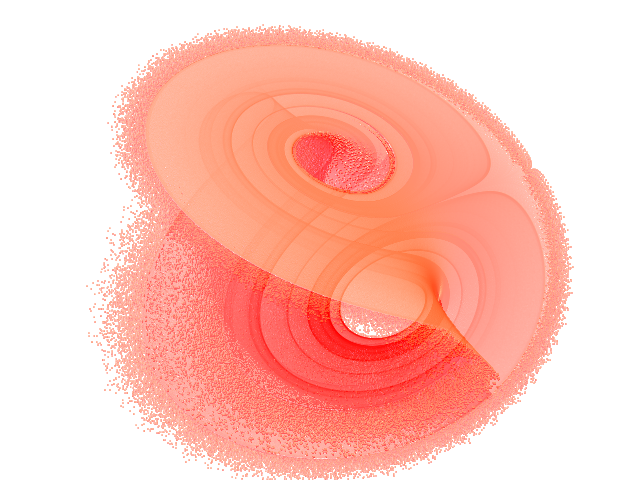
\includegraphics[scale=0.45]{lorenz.png}
\end{center}
The Lorenz system is the prototypical example of a chaotic dynamical system and has the advantage that the geometry of the attractor has been interpreted as an illusion to the butterfly effect: the attractor consists of two \enquote{wings}, resembling a butterfly, and small deviations in starting conditions can result in the trajectory being sent to the other wing of the attractor at the beginning of the trajectory, thus illustrating an extreme sensitivity to initial conditions. The Lorenz attractor also illustrated how deterministic systems can be a source of seeming randomness. It is not well-understood what constitutes either sufficient or necessary conditions for the existence of strange attractors, at least to the author's knowledge at the time of writing this, with the notable exception of the Poincaré-Bendixson theorem that implies that a system arising from an autonomous differential equation needs at least three variables to admit a strange attractor. This parallels the non-existence of compact manifolds in low-dimensional settings, and we infer that our methods function better if we imagine ourselves in rather high-dimensional settings. We refer to \cite{Hilborn} for more details. Therefore, we cannot give many theoretical guarantees of why we should expect to meet strange attractors in practice or what equations produce strange attractors. However, we can note that they have arisen mostly from studying real-world examples. The Lorenz system arose from studying weather phenomena; another example is the Lotka-Volterra systems used by population biologists to model population dynamics, see \cite{Sprott}, and recently attractors have also been suggested for modeling financial data, see \cite{finance}. The way seeming randomness can arise from deterministic settings can be a comfortable assumption when modeling real-world phenomena, and we end the discussion there. We note that there exists quite a wide array of attracts; for an introduction to some of them, we refer again to \cite{Sprott}.\\\\
We will now consider some exceptional properties that make them suitable for using Takens' theorem. We have already established the existence of dense trajectories, which makes quite a difference when wanting to use single observations of time series to reconstruct a state space because we can now expect to recreate something resembling a dense subset of it as the amount of data goes towards infinity. This is, of course, wildly imprecise, but it does serve as a theoretical assurance of the reasonability of the approach. Our first theorem is the following relatively simple fact:
\begin{thm}[Filtrations of Attractors]
Let $A$ be an attractor of the dynamical system $(\varphi, \mathcal{T}, A)$ admitting a filtration with respect to $\mathcal{G}$ and let $\varphi$ be a flow satisfying the Takens property. Then $A_U=\pi_U(A)$ is an attractor in the dynamical system $(\varphi, \mathcal{T},\mathcal{X})$.
\end{thm}
This is just a matter of using continuity to handle the technicalities; compactness is directly inherited, invariance follows from the construction of the subflows $\pi_U$, and the remaining details on attraction follow from standard topological considerations - we skip the details here and refer to \cite{mathFound}. We see that attractors are very well-behaved with respect to the filtrations compared to manifolds. Therefore, we move to the next point, namely formulating Takens' theorem in the attractor setting. Since we no longer look at manifolds, we need a new concept of dimensionality. Since strange attractors often have a fractal structure, we use the following dimension:
\begin{mydefinition}{Box-Counting Dimension}
Let $A\subset \mR^n$ be a compact set. Let $\norm{x}_{\infty}=\max_ i |x_i|$ for $x=(x_1,\ldots,x_n)\in \mR^n$. We then say that $B$ is a \emph{box} of length $\varepsilon>0$ if there exists $x_0\in \mR^n$ such that $$B=\{x\in \mR^n\mid \norm{x-x_0}_{\infty}\leqslant \varepsilon \}$$
Let then $N(\varepsilon)$ be the minimum number $N$, satisfying that there exists $N$ boxes $B_1,\ldots,B_N$ of length $\varepsilon$ such that
$$A\subset \bigcup_{m\in\{1,\ldots,N\}} B_m$$
If $-\log(\varepsilon)^{-1}\log N(\varepsilon)$
converges as $\varepsilon \to 0$, then we define the \emph{box-counting dimension} or the \emph{Minkowski-Bouligand dimension} as
$$\dim_{\text{box}}\coloneqq \lim_{\varepsilon\to 0}\frac{\log N(\varepsilon)}{\log(1/\varepsilon)}$$
\end{mydefinition}
It takes a significant amount of work, but it is possible as a reality check to show that a manifold of dimension $d$ has box-counting dimension $d$. Hence, this dimension is consistent with the natural one on manifolds. In general, the box-counting dimension is beneficial when working with fractals and sets of which we do not require a significant amount of structure. However, it turns out that it is all we need for our purpose. We refer to \cite{Fractals} for more details on fractal sets and box-counting dimensions. Meanwhile, with the box-counting dimension, we can give the following generalization of Takens' theorem in the form of a prevalence theorem of \cite{Sauer1991}:
\begin{thm}[Takens' Theorem, Version 4]\label{v4}
Let $U\subset \mR^k$ be open, let $A\subset U$ be a compact subset of $U$ with $\dim_\text{box}(A)=d$ and let $n>2d$ be an integer. If $\varphi\in\text{Diff}^1(U)$ and
\begin{enumerate}[label=\arabic*)]
	\item for every positive integer $p\leqslant n$, the set $A_p$ of periodic points of period $p$, i.e.
	$$A_p\coloneqq \left\{a\in A\mid \varphi^p(a)=a\right\}$$
	satisfies $\dim_\text{box}(A)<p/2$,
	\item if $a$ is any such periodic point with period $p\leqslant n$, then the eigenvalues of $\varphi^p$ at $a$ are all distinct.
\end{enumerate}
or if $(\varphi^t)_{t\in \mR}$ is a $C^1$ flow on U with $\varphi=\varphi^1$ and satisfy
\begin{enumerate}[label=\arabic*)]
	\item $A$ contains a finite number of equilibria, i.e.
	$$\abs{\left\{a\in A\mid \forall
	 t\in \mR: \varphi^t(a)=a\right\}}<\infty$$
	 \item there are no periodic points of period $1$ or $2$ of $\varphi$,
	\item for every positive integer $p\leqslant n$, the set $A_p$ of periodic points of period $p$ of $\varphi$ is finite,
	\item if $a$ is any such periodic point with period $p\leqslant n$, then the eigenvalues of $\varphi^p$ at $a$ are all distinct.
\end{enumerate}
then for almost every $y\in C^1(U,\mR)$, the map $\Phi_{(\varphi,y)}:M\to \mathbb{R}^{2m+1}$ defined by
$$\Phi_{(\varphi,y)}(x)=(y(x),y(\varphi(x)),...,y(\varphi^{2m}(x))),$$
is
\begin{enumerate}[label=\roman*)]
	\item injective on $A$,
	\item an immersion on each compact subset $C$ of a $C^1$ manifold contained in $A$.
\end{enumerate}
\end{thm} 
An updated version of Takens' theorem allows us to formulate an attractor version of our identifiability result of the previous section. We note here that we do not have a genericity result proving that it is a generic property that a flow satisfying the Takens property with respect to a filtration satisfies the conditions for Takens theorem on each subsystem. Such a statement is conjectured in \cite{mathFound}. We formulate our result as follows:
\begin{thm}[Identifiability in Dynamical Systems on Attractors]
Let $(\varphi, \mR,A)$ be a dynamical system, where $A$ is an attractor of box-counting dimension $d$ admitting a filtration $(A_U,\pi_{UV})_{\an(\mathcal{G)}}$ fully resolving $A$, and $(\varphi^t)_{t\in \mR}$ is a $C^1$ flow on $\mR^n$ satisfying the Takens property. Let now $U,V\in\an( \mathcal{G})$, and assume that $(A_U,\varphi_U^T)$ and $(A_V,\varphi_V^T)$ satisfy the conditions to Theorem \ref{v4} for some fixed $T\neq 0$. Let $d_U=\dim_{\text{box}}(A_U), d_V=\dim_{\text{box}}(A_U)$.\\
It now holds for almost every $C^1$ observation function $y_1:A_U\to\mR$ and and almost every $C^1$ observation function $y_2:A_V\to \mR$, with $k_1\geqslant 2d_U$ and $k_2\geqslant 2d_V$, that the delay embedding $\Phi_{(\varphi^T,y_i,k_i)}$ defined as in the expression \ref{delayemb} is an embedding of $A_U$ for $i=1$ and of $A_V$ for $i=2$. Let then 
$$A_i=\Phi_{(\varphi^T,y_i,k_i)}(A)$$ 
be the state space reconstructions for $i=1,2$ for generic and proper observation functions $y_1,y_2$. It then holds that:
\begin{enumerate}[label=\roman*.]
	\item $U\subset V$ if and only if there exists a map
	$$\Pi_{1,2}:A_2\to A_1$$ 
	that is a surjection from the union of all smooth manifolds embedded in $A$, $\bigcup M_1\subset A_1$, to the union of all smooth manifolds embedded in $\bigcup M_2\subset A_2$, and continuous when restricted to any compact subset of a smooth manifold embedded in $A_2$.
	\item $U=V$ if and only if there exists  an injective map
	$$\Psi_{1,2}:A_1\to A_2$$
	that is a bijection from the union of all smooth manifolds embedded in $A_1$, $\bigcup M_1\subset A_1$, to the union of all smooth manifolds embedded in $A_1$, $\bigcup M_2\subset A_2$ and a homeomorphism when restricted to a compact subset of a smooth manifold embedded in $A_1$.
\end{enumerate}
\end{thm}
The proof is very similar to the one we already covered. By the stable manifold theorem, we know that for each point $a$ in an attractor $A$ of a dynamical system generated by an autonomous differential equation, a stable manifold is embedded in $A$. Let us denote this manifold by $W(a)$. Strengthening the \enquote{faithfulness} assumptions on an attractor to the following:
Before that, we strengthen our notion of a fully resolved attractor in line with \cite{mathFound}
\begin{mydefinition}{Strongly Resolved Attractor}
The dynamical system ($A,\varphi$) has a \emph{strongly resolved attractor filtration with respect to $\mathcal{G}$} if the following two conditions are met:
\begin{enumerate}[label=\arabic*)]
	\item If $U$, $V$ are ancestral sets, and $U\subset V$, then there is no map $\pi_{UV}:A_U\to A_V$ that is surjective on $\bigcup_b W_V(b)\subset A_V$ when restricted to $\bigcup_a W_U(a)\subset A_U$.
	\item If $U,V$ are ancestral sets and $U\not\subset V$, $V\not\subset U$, then there is no surjection $f:\bigcup_{a} W_U(a)\to\bigcup_b W_V(b)$ that is also continuous when restricted to any compact subset of $W_U(a)$ for some $a\in A_U$.
\end{enumerate}
\end{mydefinition}
This allows for the following procedure:
\begin{cor}
Let $\varphi$ be an SCDM and $UL_\varphi$ be the corresponding lattice. Assume that assumptions I1)-I4) are fulfilled for all elements in $UL_\varphi$. Then the following algorithm recovers the transitive closure of the component graph $CG_\varphi$:
\begin{enumerate}[label=\roman*.]
	\item Let the set of variables be the set of vertices in a graph we will call \emph{RG}.
	\item For every variable $x$, build the reconstructed attractor $A_x\coloneqq \Phi	_{(\varphi^T,x,k)(A)}$.
	\item For every pair $x$ and $y$, draw an edge $x\to y$ if there exists a surjection
	 $$f:\bigcup_a W_1(a) \to \bigcup_a W_2^u(b)$$ 
	 that is continuous on any $C\subset W_1(a)$.
\end{enumerate}
Then, this will recuperate the transitive closure of $\mathcal{G}$.
\end{cor}
This is the extent to which we will follow this theoretical trail. It has become quite complicated, and in the lack of more specific theoretical results, we have to assume a lot of structure away. Nonetheless, it does provide a fairly general framework in the presence of attractor sets. There is only one piece of the puzzle missing. Usually, we will not get access to realizations of many different starting conditions but only one trajectory. This is problematic in principle: if we are trying to infer from reconstructed manifolds, we have problems.

\section{Ergodic Theory}
If we want to talk about the behavior of a single trajectory in the state space, we have to introduce some ergodic theory. The anchor is the following definition:
\begin{mydefinition}{Invariant and Ergodic Measures}
If $f:X\to X$ is a homeomorphism, $\mu$ is an \emph{invariant $f$-measure} if for all $A\subset X$ $\mu(f(A))=\mu(A)$.\\[5pt]
An invariant measure $\mu$ is called \emph{ergodic with respect to $f$}, if it is true for all $f$-invariant sets $A\subset X$ that either $\mu(A)=0$ or $\mu(X\setminus A)=0$.\\[5pt]
We define the \emph{support} of a Borel measure $\mu$ as:
$$\supp \mu=\{x\in X\mid \mu(U)>0 \text{ for } x\in U, U \text{ open }\}$$
\end{mydefinition}
There are two key results of this theory that we record here:
\begin{thm}[Krylov-Bogolubov Theorem]
Any continuous map $f$ on a metrizable compact space has an ergodic invariant Borel probability measure.
\end{thm}
\begin{thm}[Birkhoff Ergodic Theorem]
Let $T:(X,\mu)\to (X,\mu)$ be a measure preserving transformation, and let $\varphi\in L^1(T,\mu)$. Then for $\mu$-almost $x\in X$ the following time-average exists:
$$\lim_{n\to\infty}\frac{1}{n}\sum_{k=0}^{n-1}\varphi(T^k(x))$$
and we denote it $\varphi_T(x)$. In particular, if $A\subset X$ is measurable, with $\mu(A)<\infty$, and $1_A$ is the indicator function of $A$, then
$$\lim_{n\to\infty}\frac{1}{n}\sum_{k=0}^{n-1}1_A(T^k(x))=\mu(A)$$
\end{thm}
For proofs, we refer to \cite{Katok}. It thus follows that for any flow on a manifold, then on the support of an ergodic invariant Borel probability measure, all orbits of $f$ are dense in this space. If we thus assume our objects to be reasonably well-behaved on the support of an ergodic invariant Borel probability measure, then we would, in principle, use a single observation when having sufficient amounts of data. In particular, if a flow arises from a gradient field, that is, the vector field $F$ is the gradient of the scalar function $\varphi: \mathcal{U}\subset \mR^n\to \mR$, then the corresponding measure $\mu$ of a time $t$-map has support on the entirety of $\mathcal{U}$. In general, the torus is the only compact surface free of fixed points of a $C^2$ flow - and, thereby, the only compact manifold where every orbit is dense. This illustrates the need to move to attractor sets. (Theorem 14.3.1 \cite{Katok}). On the other hand, under some fairly general assumptions, it is possible to prove the existence of a global attractor.

Gibbs measure.


\chapter{Convergent Cross Mapping}\label{chapTaken}
This chapter presents a thorough account of the Convergent Cross Mapping (CCM) approach of \cite{Sugihara} and its alternatives and extensions. Notably, we discuss the methods suggested by \cite{Ye2015} and \cite{Leng2020}, which address problems not resolved by CCM, respectively, that of distinguishing bidirectional causality and unidirectional causality in systems with some degree of synchronicity and identifying the causal chain in a system knowing the causal directions between causally related variables. We will also cover some related methods that are more rooted in machine learning but still use state space reconstruction for causal inference, albeit with a less explicit theoretical foundation. We will then revisit and analyze the California Current example using the developed theory. However, it is crucial to remember that the theory of this chapter applies only to purely deterministic systems, and real-world examples often have a mix of deterministic and stochastic structures. In subsequent sections, we will address this limitation by considering a setup to replace systems of differential equations with systems of stochastic differential equations and analyze the effect of measurement noise or stochastic influences on the effectiveness of our methodology.
Meanwhile, we can exploit this idea of information being encoded in effect variables to great effect: This allows us to reformulate causality from the point of view of deterministic systems. The principle itself is fairly simple, but we do require some technical assumptions to make the theory work, which is not in any way empirically motivated nor entirely interpretable but fare under what we usually consider regularity assumptions - a sweep-it-under-the-rug-interpretation would be that we just assume the data to be reasonably well-behaved. 
\url{https://besjournals.onlinelibrary.wiley.com/doi/10.1111/2041-210X.13150}

\section{Implementation}
We will cover different approaches to the implementation of the algorithms in practice. Consider two time series of length $L$:
$$X=(X(1),\ldots, X(L)), Y=(Y(1),\ldots, Y(L))$$
For a fixed embedding dimension $E$, we form the lagged coordinate vectors of $x$:
$$x(t)=(X(t), X(t-\tau),X(t-2\tau),\ldots, X(t-(E-1)\tau))$$
for $t=1+(E-1)\tau$ to $t=L$. We denote by
$$M_X\coloneqq\{x(t)\mid t\in \{1+(E-1)\tau,\ldots,L\}\}$$
the \emph{shadow manifold of $X$}. We then move to the prediction of $Y(t)$ for $t\geqslant 1+(E-1)\tau$:
\begin{enumerate}[label=\arabic*.]
	\item First we take $t_1,\ldots,t_{E+1}$ to be the $E+1$ numbers in succession (closest to farthest) for which $\norm{x(t)-x(t_{i})}$ is minimized (randomized order in case of a tie).
	\item We then compute the score of each chosen element
	$$u_i=\exp\left(-\frac{\norm{x(t)-x(t_i)}}{\norm{x(t)-x(t_1)}}\right)$$
	\item We then compute the weight of the $t_i$'th observation
	$$w_i=\frac{u_i}{\sum_{j=1}^{E+1} u_j}$$
	\item We then compute the estimate
	$$\hat{Y}(t)|M_X=\sum_{i=1}^{E+1} w_i Y(t_i)$$
\end{enumerate}
We then measure the cross-map skill as the correlation between the estimates of $Y$ and the actual values.\\[5pt]
The reasoning here is that if $X$ contains the dynamics of $Y$, the value at time point $t$ must be revealed by the position on the manifold. This can be estimated by the $k$-nearest neighbors when the attractor is sufficiently filled in - and this has the added advantage of dealing with observational noise. This is also what is suggested by \cite{Casdagli}. As the time-series length increases, we should observe convergence towards the true value. There are two heuristics to consider: the choice of embedding dimension and time lag. For the embedding dimension, we can use a similar heuristic. Instead of predicting $Y(t)$, we can try to predict $X(t+1)$ in the same manner and look at the prediction skill as a function of the embedding in dimension. 

\subsection*{Reference Model}
We will reference the following model built on a multivariate Ornstein-Uhlenbeck process. More specifically, we will consider the following setup. Let the $d$-dimensional stochastic process $X_t$, $t\geqslant 0$, be given by the following stochastic differential equation
$$dX_t=M X_t\ dt+\rho I_d\ dW_t$$
with $W_t$ a $d$-dimensional  Brownian motion, $M$ a $d\times d$ drift matrix, and $\rho\in \mathbb{R}$ a scalar. We will then consider observations at time points $0\leqslant t_1<t_2<\cdots <t_n$, $n\in \mathbb{N}$, with some observation noise
$$Y_{t_i}=X_{t_i}+\xi_i,\quad i=1,...,n$$
where $\xi_i$ is iid with $\mathbb{E} \xi_i=0$ and $V(\xi_i)=\sigma^2$ for some variance parameter $\sigma^2\in \mathbb{R}_{\geqslant 0}$. Interesting variations of this model are $\sigma^2=0$, implying no observation noise, and $\rho=0$, which removes the stochasticity of the process.
\section{Direct Extensions}


\section{Machine Learning Extensions}
\url{https://arxiv.org/pdf/nlin/0405016.pdf}\\[5pt]
\url{file:///C:/Users/rasmu/Downloads/s41598-021-87316-6.pdf}\\[5pt]
\url{https://static-content.springer.com/esm/art%3A10.1038%2Fs41598-021-87316-6/MediaObjects/41598_2021_87316_MOESM1_ESM.pdf}

\section{Dynamical Systems under Noise}
Consider the following generalization of the Ornstein-Uhlenbeck process:
$$du(t)=-Au(t)\ dt+F(u(t))\ dt+B u(t)\ dW_t,\quad t\geqslant 0$$
with the following assumption on $F:H\to H$. We can then do a stable manifold theorem for this setting as well.
\cite{StableManifoldStoc} 


\section{Simulation Study}
\url{https://pure.au.dk/portal/files/136561486/Causal_inference_from_noisy_time_series_data_AM17.pdf}




\bibliographystyle{apalike2}
\bibliography{kilder}
\end{document}
